\documentclass[a4paper,12pt,english]{report}
\usepackage[utf8]{inputenc}
\usepackage[T1]{fontenc}
\usepackage[english]{babel}
\usepackage{amsmath}
\usepackage{makeidx}
\usepackage{setspace}
\usepackage{array}
\usepackage{graphicx}
\usepackage{wrapfig}
\usepackage{lscape}
\usepackage{rotating}
\usepackage{epstopdf}
\usepackage{subcaption}
\usepackage{float}
\usepackage{eurosym}
\usepackage[top=3cm, bottom=3cm, left=1.5cm, right=2cm]{geometry}
\usepackage{pdfpages}
\usepackage{fancyhdr}
\pagestyle{fancy}
\usepackage{hyperref}
\usepackage{array,multirow,makecell}
\setcellgapes{3pt}
\setlength{\parindent}{1.1cm}
\makegapedcells
\newcolumntype{R}[1]{>{\raggedleft\arraybackslash }b{#1}}
\newcolumntype{L}[1]{>{\raggedright\arraybackslash }b{#1}}
\newcolumntype{C}[1]{>{\centering\arraybackslash }b{#1}}
\renewcommand{\footrulewidth}{1pt}
\fancyfoot[C]{\textbf{\thepage}}
\fancyfoot[R]{Academic Year: 2024/2025}
\fancyfoot[L]{ENSIAS}

\usepackage{blindtext}
\begin{document}

% \pagenumbering{gobble} % Supprimer la numérotation des pages

\begin{titlepage}
\begin{center}

\begin{minipage}{.2\textwidth}%

\includegraphics[width=.8\textwidth]{images/ensias}
 \end{minipage}%
 \hfill
 \begin{minipage}{.33\textwidth}%
 \centering
 
\includegraphics[width=0.8\textwidth]{./images/renault_digital}
 \end{minipage}%
 \hfill
 \begin{minipage}{.2\textwidth}%
 
\includegraphics[width=\textwidth]{images/um5}
 \end{minipage}
 

\textsc{\large National School of Computer Science and Systems Analysis - RABAT \\ [0.2cm] Web and Mobile Engineering Department}\\[0.8cm]

% Title
\begin{figure}[H]
    \begin{center}
        \large Program : IDSIT
    \end{center}
\end{figure}

{\LARGE \bfseries Second Year Internship\\[2cm]}

\textcolor{black}{\rule{\textwidth}{2pt}}\\[0.5cm]

{\LARGE \bfseries Automation of the Audit/Alert Process for Expirable Cryptographic Resources\\ [0.5cm]
}

\textcolor{black}{\rule{\textwidth}{2pt}}\\[0.5cm]
\vspace{2cm}

% Author and supervisor
\begin{minipage}{0.36\textwidth}
\begin{flushleft} \large
\emph{Carried out by:}\\[0.4 cm]
\textsc{Mohammed} FADLOUALLAH\\
\end{flushleft}
\end{minipage}
\begin{minipage}{0.6\textwidth}
\begin{flushleft} \large
\emph { \hspace*{1.3cm}Defended on ??/10/2025 before the Jury:} \\[0.4 cm]
\hspace*{1.3cm} Pr. Lorum IPSUM \\ \hspace*{1.3cm} Pr. Lorum IPSUM
\end{flushleft}
\end{minipage}
\vspace{1.3cm}

\begin{minipage}{0.36\textwidth}
\begin{flushleft} \large
\end{flushleft}
\end{minipage}
\begin{minipage}{0.63\textwidth}
\begin{flushleft} \large
\emph{ \hspace*{1.3cm} Supervised by:}\\[0.4 cm] \hspace*{1.5cm} M. Hamza TAHRI\\
\end{flushleft}
\end{minipage}

\vfill

% Bottom of the page
\vspace{1.3cm}
{\large \ Academic Year 2024/2025}

\end{center}
\end{titlepage}

\vspace*{1cm}
\begin{center}
    \textbf{\huge{Dedication}}
\end{center}
\vspace{1cm}

\begin{doublespace} 
    \large{
    \noindent
    I dedicate this work to:\\
    My mother, source of tenderness and love, for her support throughout my academic life.\\
    My father, who has always supported me and done everything possible to help me.\\
    My brothers and sisters, whom I love dearly.\\
    My extended family.\\
    My dear friends and my teachers.\\
    All the people who have collaborated closely or distantly in the development of this work.\\
    May God grant them health and prosperity.
    }
\end{doublespace}


\vspace*{1cm}
\begin{center}
    \textbf{\huge{Acknowledgments}}
\end{center}
\vspace{1cm}

\begin{doublespace}
    \large
    I would like to thank Renault Digital Morocco for this enriching internship opportunity.

    \vspace{0.5cm}

    My thanks also go to my company supervisor, Mr. Hamza TAHRI, for the interest he showed in supervising this project. His enriching remarks and wise advice were of great help throughout this work.

    \vspace{0.5cm}

    I also thank all the members of the KMS team for welcoming me warmly, accompanying me with kindness, and supporting me in understanding the technical aspects of the project. Their availability, team spirit, and expertise greatly contributed to the success of this professional experience.

    \vspace{0.5cm}

    I also wish to express my sincere thanks to the entire teaching staff of the school for the quality of their teaching and their dedication to my education. Their diverse and complementary expertise contributed to enriching my academic journey and preparing me for my future professional life.

    \vspace{0.5cm}

    Finally, I express my gratitude to all the people, near and far, who contributed to making this internship a formative and motivating step in my career.
\end{doublespace}



\vspace*{1cm}
\begin{center}
    \textbf{\huge{Abstract:}}
\end{center}
\vspace{1cm}

\begin{doublespace}
This internship report presents the development of an automated notification system for the Key Management System (KMS) at Renault Digital Morocco. The project addresses the critical need for proactive management of expiring cryptographic resources within Renault Group's security infrastructure.\\

The main objective was to design and implement an intelligent notification system that automatically identifies expiring certificates and keys, and delivers targeted alerts to responsible stakeholders through multiple communication channels. The system prevents service disruptions by providing early warnings before cryptographic resource expiration.\\

The solution was developed using Agile methodology with Java Spring Boot framework. The implementation includes automated resource discovery, role-based notification targeting, multi-channel delivery via email and real-time in-app notifications, and comprehensive audit trail capabilities. The system integrates seamlessly with the existing KMS database architecture.\\

Testing validated the system's ability to reliably identify expiring resources, deliver notifications through REST APIs and WebSocket connections, and maintain operational continuity. The implemented solution transforms reactive resource management into a proactive, automated process, enhancing security compliance and reducing operational risks.\\

\noindent
\textbf{Keywords:} Key Management System, Cryptographic Resources, Automated Notifications, Spring Boot
\end{doublespace}

\vspace*{1cm}
\begin{center}
    \textbf{\huge{List of Abbreviations}}
\end{center}
\vspace{1cm}

\begin{doublespace}
    \begin{center}
        \begin{tabular}{|l|l|}
            \hline
            \textbf{Abbreviation} &  \textbf{Definition} \\

            \hline
            API & Application Programming Interface \\

            \hline
            CI/CD & Continuous Integration/Continuous Deployment \\

            \hline
            CRUD & Create, Read, Update, Delete \\

            \hline
            DLQ & Dead Letter Queue \\

            \hline
            HTTP & HyperText Transfer Protocol \\

            \hline
            IDE & Integrated Development Environment \\

            \hline
            JPA & Java Persistence API \\

            \hline
            JSON & JavaScript Object Notation \\

            \hline
            KMS & Key Management System \\

            \hline
            PKI & Public Key Infrastructure \\

            \hline
            REST & REpresentational State Transfer \\

            \hline
            SMTP & Simple Mail Transfer Protocol \\

            \hline
            SQL & Structured Query Language \\

            \hline
            TTL & Time To Live \\

            \hline
            URL & Uniform Resource Locator \\
            
            \hline
        \end{tabular}
    \end{center}
\end{doublespace}

\listoffigures

\renewcommand{\contentsname}{Table de matières}
\setcounter{tocdepth}{2}
\tableofcontents

\cleardoublepage
\pagenumbering{arabic} % Commencer la numérotation des pages à partir de la 8ème page en chiffres arabes
\setcounter{page}{9}


\addcontentsline{toc}{chapter}{General Introduction}
\fancyhead{}  % Efface tous les en-têtes existants

\vspace*{1cm}
\begin{center}
    \textbf{\huge{General Introduction}}
\end{center}
\vspace{1cm}

\begin{doublespace}
In today's digital landscape, cybersecurity has become a cornerstone of enterprise operations, particularly in the automotive industry where connected vehicles require robust cryptographic protection. The management of cryptographic resources—certificates and keys that secure communications—presents a critical challenge for organizations seeking to maintain both security and operational continuity.

The Renault Group has recognized the strategic importance of centralizing cryptographic asset management through its Key Management System (KMS) initiative. While secure storage and distribution of cryptographic materials forms the foundation of this system, proactive lifecycle management represents an equally crucial dimension that can prevent service disruptions and security vulnerabilities.

This internship project addresses a fundamental gap in automated cryptographic resource management: the need for intelligent notification systems that can anticipate expiration events and coordinate appropriate organizational responses. The challenge extends beyond simple monitoring to encompass sophisticated stakeholder targeting, multi-channel communication, and seamless enterprise integration.

The work presented details the design and implementation of an automated audit and alert system that transforms reactive resource management into a proactive, intelligence-driven process. Through modern software engineering practices and enterprise-grade technologies, this solution enhances security compliance while reducing operational overhead and risk exposure.

This document chronicles the journey from problem analysis through system design to practical implementation, demonstrating how targeted automation addresses complex organizational challenges in cybersecurity management.
\end{doublespace}

\setcounter{chapter}{1}
\fancyhead[L]{Chapter I}
\fancyhead[R]{General project context}

\vspace*{9cm}
\begin{doublespace}
    \centering
    \addcontentsline{toc}{chapter}{Chapter I: Work context}
    \textbf{ \huge Chapter I \\ [1 cm] General project context}
\end{doublespace} 

\newpage
\fancyhead[R]{\rightmark}

\doublespacing

\section*{Introduction}

This chapter presents the general context of the project, beginning with an overview of Renault Group and its Moroccan subsidiary, Renault Digital Morocco. It then introduces the Key Management System (KMS) project and the specific challenges related to cryptographic resource lifecycle management. Finally, it outlines the project objectives, management methodology, and planning approach used throughout the development process.

\section{Presentation of Renault}

\subsection{Renault Group}
The \textbf{Renault Group} is a major French company that designs and manufactures cars and commercial vehicles, with a history dating back to 1899. Today, it operates globally and brings together well-known brands such as Renault, Dacia, Alpine and Mobilize. \\

\noindent
The \textbf{Renault Group} was founded in 1899 by Louis Renault and his brothers, and quickly became known for its spirit of innovation and ability to mass produce in the automotive industry. The company played an important role during both world wars, was nationalized in 1945, then privatized in 1996. In 1999, Renault formed a strategic alliance with Nissan and expanded internationally by acquiring brands such as Dacia and Samsung Motors, with a desire to strengthen itself in global markets and modernize its operations.


\subsection{Renault Group Morocco}
\textbf{Renault Group Morocco} is a key player in the automotive industry in Morocco, with two major production sites: the SOMACA plant in Casablanca and the Tangier plant.
In addition to these two production sites, Renault Group Morocco relies on a well-integrated ecosystem composed of five key entities, each playing an essential role in the group's success, both locally and internationally.


\begin{figure}[H]
    \centering
    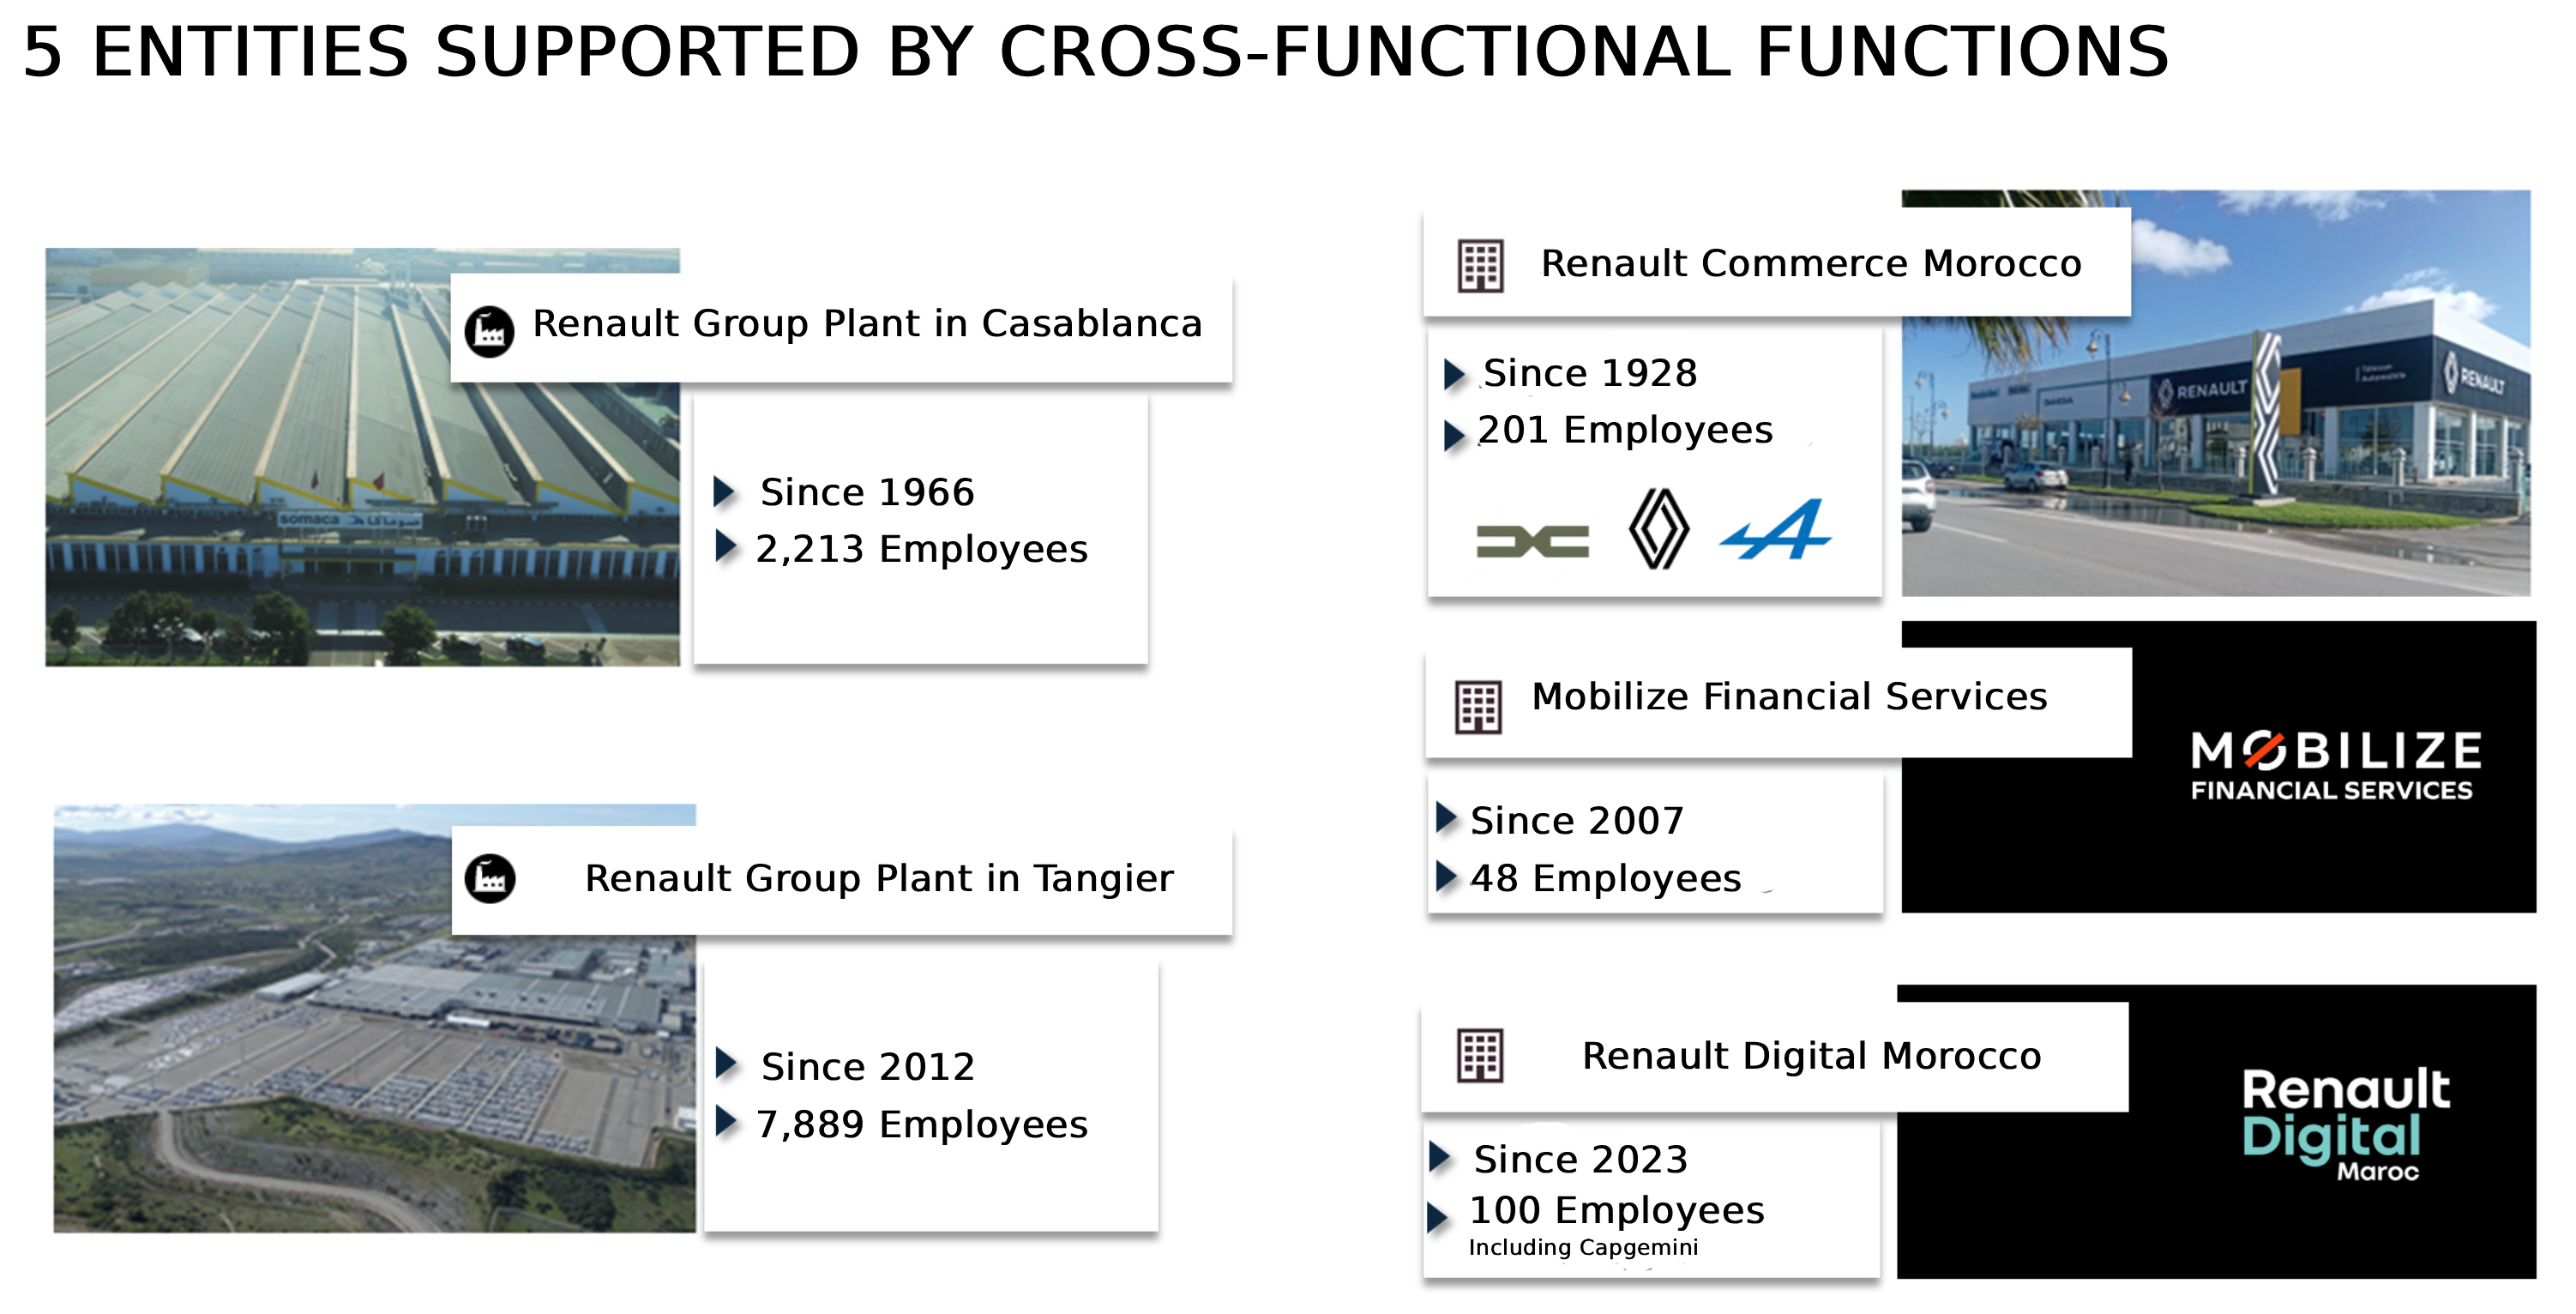
\includegraphics[width=1\linewidth]{images/renault's_entities.png}
    \caption{Entities of Renault Group Morocco}
\end{figure}

\subsection{Renault Digital Morocco}
\textbf{Renault Digital Morocco} (also called RDM) is a subsidiary of the Renault Group that supports the group in its digital transformation. RDM focuses on the development and maintenance of digital projects for all business sectors of the company and its suppliers worldwide, covering areas ranging from design and manufacturing to marketing and after-sales.



\section{Project presentation}

\subsection{General project context}
In a context where cybersecurity is becoming a major issue for the automotive sector, the Renault Group has undertaken the development of a centralized cryptographic key management system, called \textbf{Key Management System (KMS)}. This project is part of a desire to strengthen the company's security posture, while ensuring compliance with international standards and regulatory requirements of the sector.

\noindent
The \textbf{KMS} has the main objective of centrally managing all cryptographic keys used within the Renault Group, by offering:
\begin{itemize}
    \item Compliance with international regulations and cryptographic key management best practices.
    \item Enhanced security of vehicles through the management of the lifecycle of cryptographic objects.
    \item Implementation of new automated uses such as key exchange, their diversification by vehicle, or inventory management.
\end{itemize}

\noindent
The system consists of several complementary modules:
\begin{itemize}
    \item \textbf{KMS Client Module}: a REST API that securely exposes cryptographic operations to internal applications and suppliers;
    \item \textbf{CipherTrust Appliances}: hardware equipment ensuring secure storage and cryptographic operations;
    \item \textbf{KMS Web Portal}: a web interface allowing key management, access rights management, as well as inventory visualization;
    \item \textbf{KMS Admin Module}: intermediate module between the web portal and cryptographic equipment, ensuring notably signature requests to the PKI.
\end{itemize}

\newpage
\section{Project management}

\subsection{Agile development method}
Agile development is an iterative and incremental approach for project management and software development. The development team delivers iteratively and incrementally based on the priority of user needs. In agile development, a project is divided into several sub-projects before development. Each sub-project is tested and integrated, and it must also be visible and usable before delivery.\\

\noindent
Agile development allows the development team to continuously deliver products, reduce risks, constantly improve the quality of team development, be flexible to changes in user needs and improve customer satisfaction in an iterative development process.

\subsection{Scrum development}
Scrum is an agile development framework and an incremental and iterative development process. The Scrum team consists of a development team, the Scrum Master and the Product Owner (PO).\\

\noindent
With the agile development method, all client needs are considered as User Stories (US). They are provided by the PO. All US are listed in the Product Backlog with its priority given by PO. The development team delivers incrementally and iteratively products according to the Product Backlog. Agile development divides the project duration into Sprints. Before development, the development team and the PO determine the Sprint cycle. The development team estimates its velocity. After each Sprint Planning, the development team chooses User Stories for this Sprint based on its velocity and the priority of User Stories. The development team delivers the products developed in this Sprint after each Sprint, and reviews this Sprint to improve the development quality of the next Sprint.

\subsection{Scrum Board}

The \textit{Scrum Board} is a visual board that represents the progress of tasks during a sprint. 
It is divided into several columns representing the different states of a task, from its planning to its completion. 
Each task is materialized by a ticket that moves from left to right as it progresses.  

\noindent
A typical example of a Scrum Board includes the following columns: 
\textbf{To Do}, 
\textbf{In Progress}, 
\textbf{Blocked}, 
\textbf{Testing/Review} and 
\textbf{Done}. 
This system provides immediate visibility on the sprint's progress, facilitates coordination between team members and helps quickly identify potential blocking points.  

\begin{figure}[H]
    \centering
    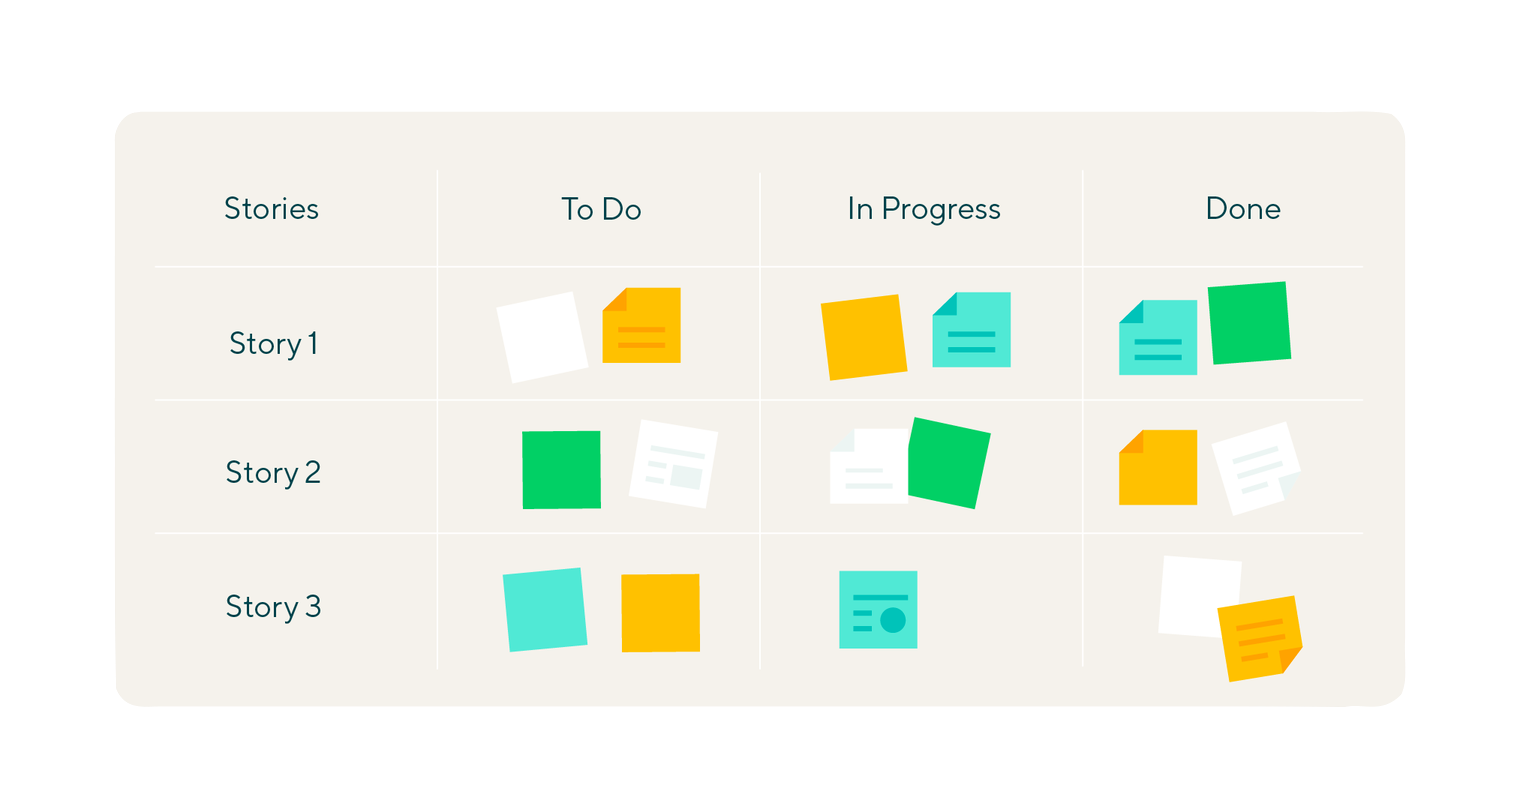
\includegraphics[width=0.8\textwidth]{images/scrum_board.png}
    \caption{Example of Scrum Board structure}
\end{figure}

In the context of this project, the \textbf{Jira} tool was used to implement the Scrum Board. 
Jira is an agile project management platform widely adopted in the industry. 
It not only allows managing tasks in the form of tickets, but also configuring \textit{workflows} adapted to the team, tracking progress via indicators (such as \textit{burndown charts}) and centralizing communication around the project.  

\begin{figure}[H]
    \centering
    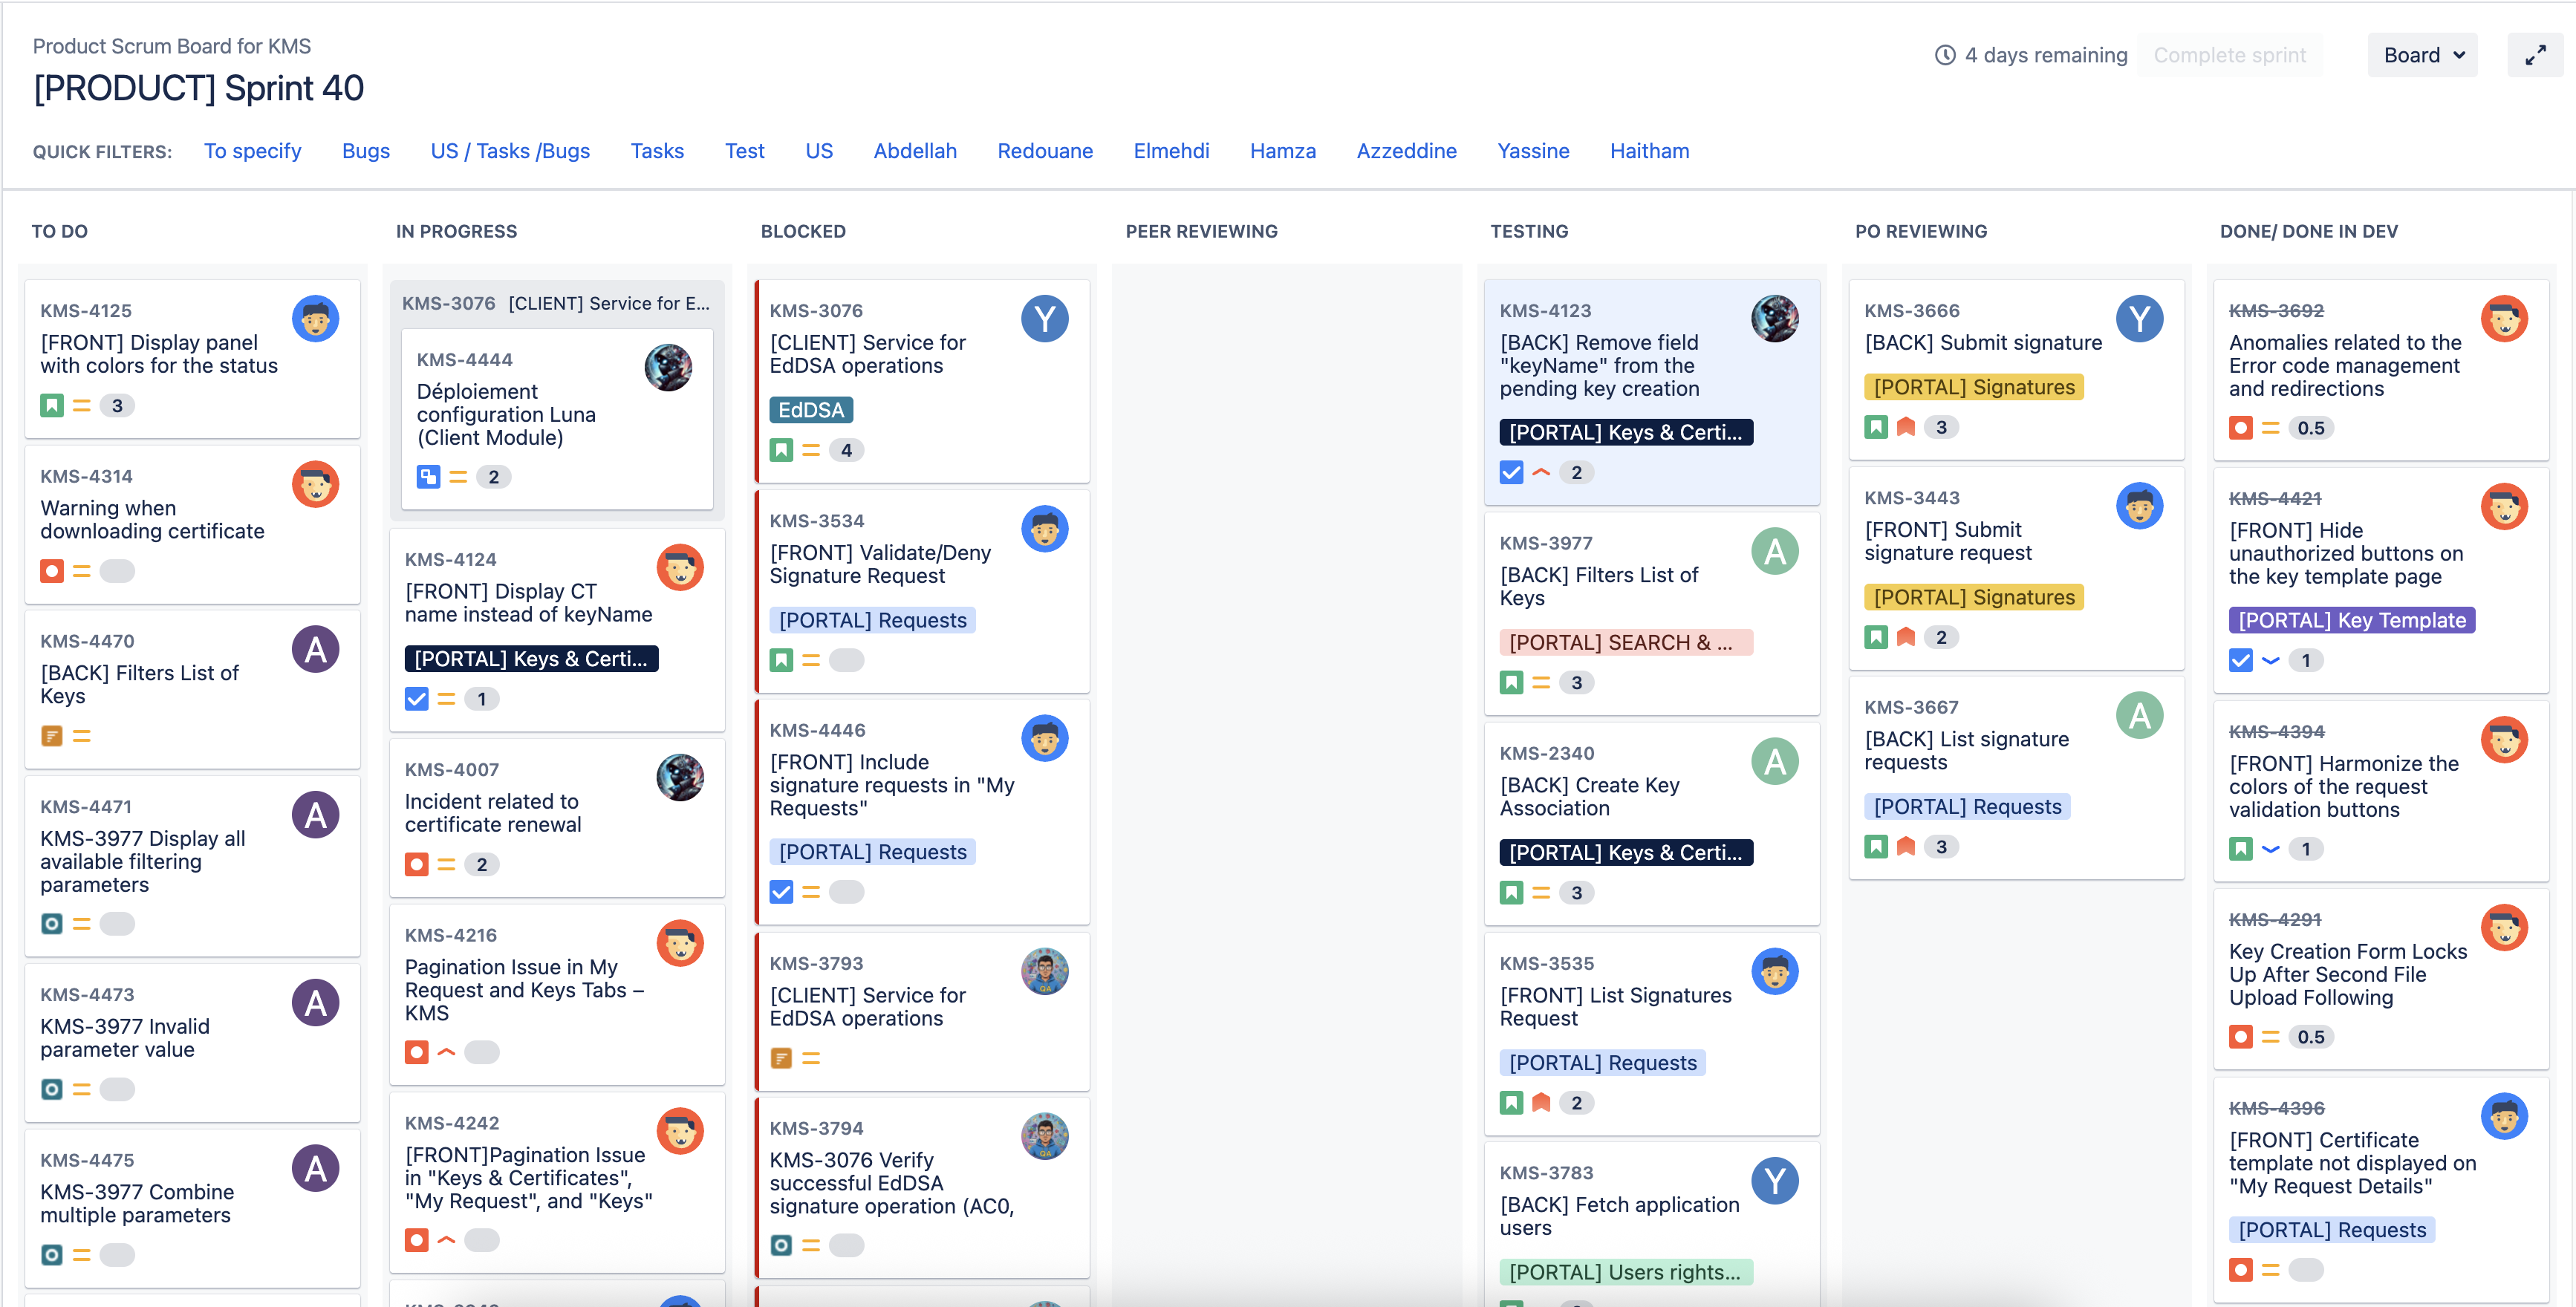
\includegraphics[width=0.9\textwidth]{images/jira_scrum_board.png}
    \caption{Real project Scrum Board under Jira}
\end{figure}

\subsection{Scrum Ceremonies}

Scrum ceremonies are regular meetings that structure the work rhythm and ensure effective communication within the team. In the context of this project, five main ceremonies were implemented:

\noindent
\textbf{Daily Meeting (Daily Standup):} A short daily meeting of 15 minutes maximum where each team member shares what they accomplished the previous day, what they plan to do today, and any obstacles they encounter. This ceremony ensures daily synchronization and rapid identification of blocking points.

\noindent
\textbf{Backlog Refinement:} Regular sessions where the Product Owner and the development team review, estimate, and prioritize User Stories in the Product Backlog. These meetings help clarify requirements, break down complex stories, and ensure that the backlog remains up-to-date and ready for future sprints.

\noindent
\textbf{Sprint Review:} A meeting held at the end of each sprint where the development team demonstrates the completed functionalities to stakeholders. This ceremony allows for immediate feedback collection and validation that the developed features meet expectations.

\newpage
\noindent
\textbf{Sprint Retrospective:} A reflection meeting where the team analyzes what went well, what could be improved, and defines concrete actions for the next sprint. This ceremony promotes continuous improvement of working methods and team dynamics.

\noindent
\textbf{Sprint Planning:} A meeting at the beginning of each sprint where the team selects User Stories from the Product Backlog and defines the sprint objective. The team estimates the effort required and commits to delivering specific functionalities within the sprint timeframe.

\section{Problematic and Objectives}

\subsection{Problem Statement}

As part of the ongoing development of the Key Management System (KMS) at Renault Group, a critical requirement has emerged for proactive management of cryptographic resource lifecycles. The KMS is being designed to centrally manage certificates, keys, and other cryptographic objects that are essential for vehicle security and internal applications.

\subsubsection{Identified System Requirements}

\textbf{Proactive Expiration Management:} The KMS needs to include functionality that proactively identifies and alerts stakeholders about upcoming certificate and key expirations. Without this capability, the system would only provide storage and management functions without preventing potential service disruptions.

\noindent
\textbf{Role-Based Notification Requirements:} The system design requires that notifications reach the appropriate personnel based on their roles and responsibilities within the organization. Different stakeholders have varying levels of responsibility for cryptographic resource management, and the notification system must account for these distinctions.

\noindent
\textbf{Multi-Channel Communication Needs:} Modern enterprise applications require multiple communication channels to ensure message delivery and user engagement. The KMS must support both formal notification channels (email) and real-time communication (in-app notifications) to meet diverse user preferences and operational requirements.

\subsection{Project Objectives}

\subsubsection{Primary Objectives}

\textbf{Implement Proactive Resource Monitoring:} Develop a notification system that automatically identifies certificates and keys approaching expiration and initiates appropriate alerts to responsible stakeholders.

\noindent
\textbf{Design Role-Based Notification Targeting:} Create a sophisticated targeting mechanism that identifies and notifies only relevant users based on their specific roles and their association with particular applications and resources.

\noindent
\textbf{Establish Multi-Channel Communication:} Implement both email and real-time in-app notification channels to ensure reliable message delivery and accommodate different user preferences and operational contexts.

\subsubsection{Secondary Objectives}

\textbf{Implement Strategic Notification Timing:} Develop a notification schedule that provides early warnings while escalating urgency as expiration approaches, balancing user awareness with notification fatigue.

\noindent
\textbf{Provide Operational Flexibility:} Include feature flag controls that allow runtime configuration of notification channels, supporting testing scenarios and phased deployment strategies.

\noindent
\textbf{Maintain Comprehensive Audit Trails:} Implement notification history tracking for compliance reporting and system monitoring, documenting when notifications were sent, to whom, and their delivery status.

\newpage
\subsection{Project Planning (Gantt Diagram)}

Our project is managed following a chronological breakdown into phases, which specifies what needs to be done (the tasks) and by whom (the resources). To represent this distribution, we use a Gantt diagram, a type of bar chart that illustrates a series of tasks over a given period. This diagram displays the list of activities to be carried out in the project, as well as their start and end dates, and constitutes a visual representation of a project schedule.

Here is an example of our Gantt diagram:

\begin{figure}[H]
    \centering
    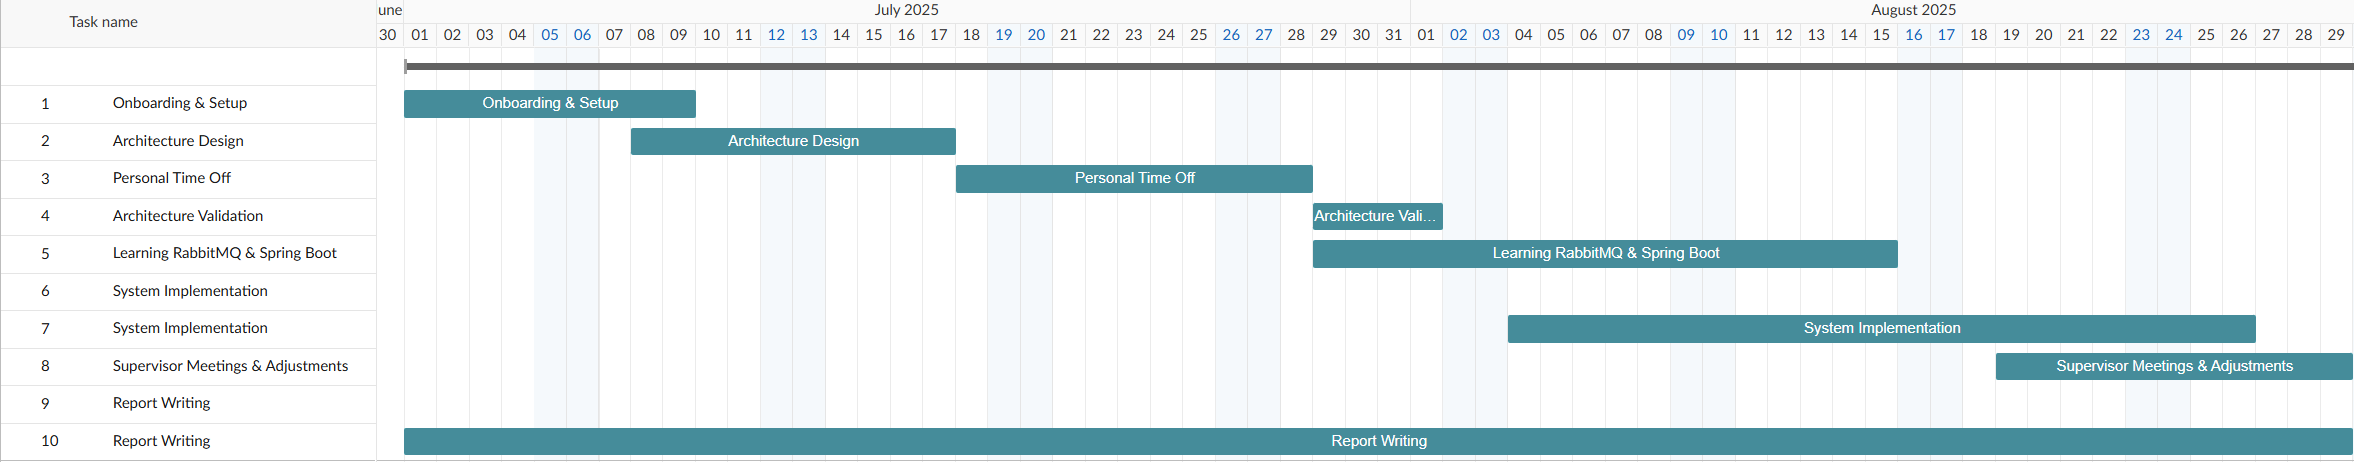
\includegraphics[width=1\linewidth]{images/gantt_diagram.png}
    \caption{Project Planning Gantt Diagram - July 1 to August 31}
    \label{fig:gantt_diagram}
\end{figure}

\section*{Conclusion}

This chapter established the foundation for understanding the project context within Renault Group's digital transformation initiative. The presentation of the KMS project highlighted the critical need for automated management of cryptographic resource lifecycles, particularly the challenge of proactive expiration monitoring and notification. The adoption of Agile methodology with Scrum framework, supported by appropriate project management tools, provides a structured approach for delivering this complex notification system that will enhance the security posture of Renault's cryptographic infrastructure.

\setcounter{chapter}{2}
\fancyhead[L]{Chapter II}
\fancyhead[R]{Analysis and Design}

\vspace*{9cm}
\begin{doublespace}
    \centering
    \addcontentsline{toc}{chapter}{Chapter II: Analysis and Design}
    \textbf{ \huge Chapter II \\ [1 cm] Analysis and Design}
\end{doublespace}

\newpage
\fancyhead[R]{\rightmark}

\setcounter{section}{0}
\section*{Introduction}

This chapter presents the analysis and design phase of the notification system for cryptographic resource management within the KMS. The analysis phase identifies the functional and non-functional requirements, while the design phase defines the system architecture, database structure, and component interactions necessary for implementing an automated audit and alert system for expirable cryptographic resources.

\section{Requirements Analysis}

\subsection{Functional Requirements}

The functional requirements describe the main features that the notification system must provide. Based on the analysis of the KMS context and user needs, the following functional requirements have been identified:

\subsubsection{Resource Discovery and Monitoring}

\textbf{Automatic Resource Detection:} The system must be capable of automatically discovering certificates and keys that are approaching their expiration date. This discovery process should scan the database daily to identify resources requiring notification.

\noindent
\textbf{Expiration Timeline Management:} The system must calculate the number of days remaining before each resource expires and maintain this information up-to-date to ensure accurate notification timing.

\noindent
\textbf{Resource Lifecycle Tracking:} The system must track the status of each resource throughout its lifecycle, from active use to expiration or renewal.

\subsubsection{Notification Management}

\textbf{Multi-Channel Communication:} The system must support multiple notification channels to ensure message delivery reliability:
\begin{itemize}
    \item Email notifications for formal communication
    \item In-app notifications for real-time alerts
    \item Configurable channel activation/deactivation
\end{itemize}

\noindent
\textbf{Role-Based Notification Targeting:} The system must identify and notify only relevant users based on their organizational roles:

\noindent
\textbf{Strategic Notification Scheduling:} The system must implement an intelligent notification schedule that provides timely alerts while minimizing notification fatigue. The timing should balance early warning with user experience.

\noindent
\textbf{Notification Status Management:} The system must track notification states throughout their lifecycle:
\begin{itemize}
    \item PENDING: notification created but not yet sent
    \item SENT: notification successfully delivered
    \item READ: user has acknowledged the notification
    \item FAILED: notification delivery failed
    \item CANCELLED: notification cancelled due to user response
    \item EXPIRED: resource has expired
    \item RENEWED: resource has been renewed
\end{itemize}

\subsubsection{User and Resource Management}

\textbf{Resource Response Tracking:} The system must allow users to mark resources as "responded to," automatically cancelling further notifications for those resources.

\noindent
\textbf{User Session Management:} For real-time notifications, the system must maintain active user sessions and route notifications to appropriate connected users.

\noindent
\textbf{Historical Tracking:} The system must maintain a complete audit trail of all notification activities for compliance and monitoring purposes.

\subsection{Non-Functional Requirements}

The non-functional requirements ensure the quality, performance, and reliability of the notification system:

\subsubsection{Performance Requirements}

\textbf{Scalability:} The system must handle a large number of users (hundreds) and resources (thousands) without performance degradation.

\noindent
\textbf{Concurrent Processing:} The system must support concurrent notification processing with configurable parallelism levels (2-5 concurrent email processing, 2-10 concurrent message processing).

\subsubsection{Reliability Requirements}

\textbf{Message Delivery Reliability:} The system must ensure reliable message delivery through:
\begin{itemize}
    \item Message queue persistence
    \item Automatic retry mechanisms with exponential backoff
    \item Dead letter queue handling for failed messages
    \item Message TTL configuration (10 minutes for email, 5 minutes for in-app)
\end{itemize}

\noindent
\textbf{Job Scheduling Reliability:} The system must ensure reliable execution of scheduled jobs:
\begin{itemize}
    \item Persistent job storage
    \item Automatic job recovery after system restart
    \item Job execution monitoring and logging
\end{itemize}

\newpage
\section{System Analysis}

\subsection{Use Case Analysis}

The use case analysis identifies the main actors and their interactions with the notification system.

\subsubsection{Main Use Cases}

% TODO: Insert Use Case Diagram here
\begin{figure}[H]
    \centering
    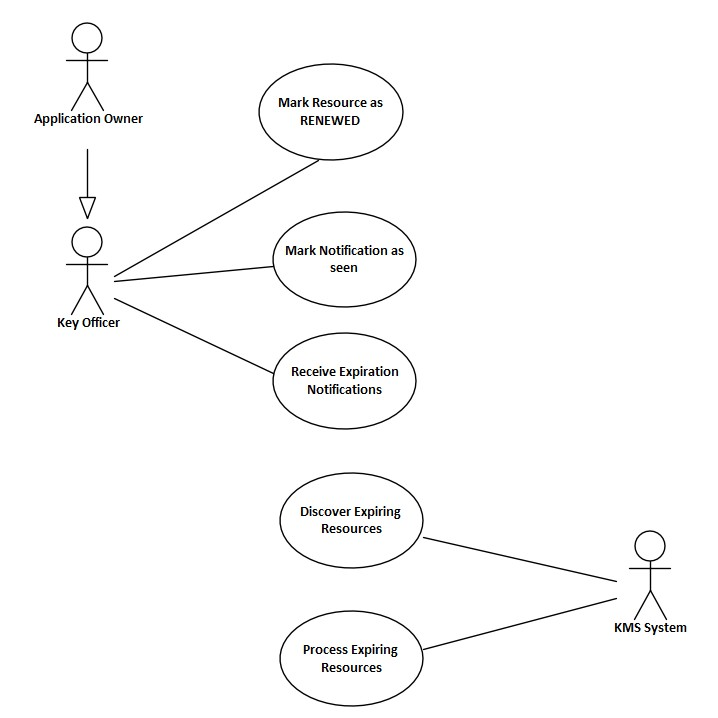
\includegraphics[width=0.8\textwidth]{images/use_case_diagram.jpg}
    \caption{Use Case Diagram - Notification System}
    \label{fig:use_case_diagram}
\end{figure}

\textbf{UC1: Receive Expiration Notifications}
\begin{itemize}
    \item \textbf{Actor:} Application Owner, Key Officer
    \item \textbf{Description:} Users receive notifications about expiring resources through email and in-app channels
    \item \textbf{Preconditions:} User has appropriate role assignment for the resource
    \item \textbf{Main Flow:} 
        \begin{enumerate}
            \item System discovers expiring resource
            \item System identifies responsible users
            \item System sends notifications via configured channels
            \item User receives and acknowledges notification
        \end{enumerate}
\end{itemize}

\noindent
\textbf{UC2: Mark Resource as Renewed}
\begin{itemize}
    \item \textbf{Actor:} Application Owner, Key Officer
    \item \textbf{Description:} Users indicate they have renewed an expiring resource
    \item \textbf{Preconditions:} User has received notification for the resource
    \item \textbf{Main Flow:}
        \begin{enumerate}
            \item User accesses notification system
            \item User selects resource to mark as renewed
            \item System cancels future notifications for the resource
            \item System updates resource status to RENEWED
        \end{enumerate}
\end{itemize}

\section{System Design}

\subsection{System Architecture}

The notification system follows a layered architecture pattern that ensures separation of concerns and maintainability.

\subsubsection{Architectural Overview}

% TODO: Insert System Architecture Diagram
\begin{figure}[H]
    \centering
    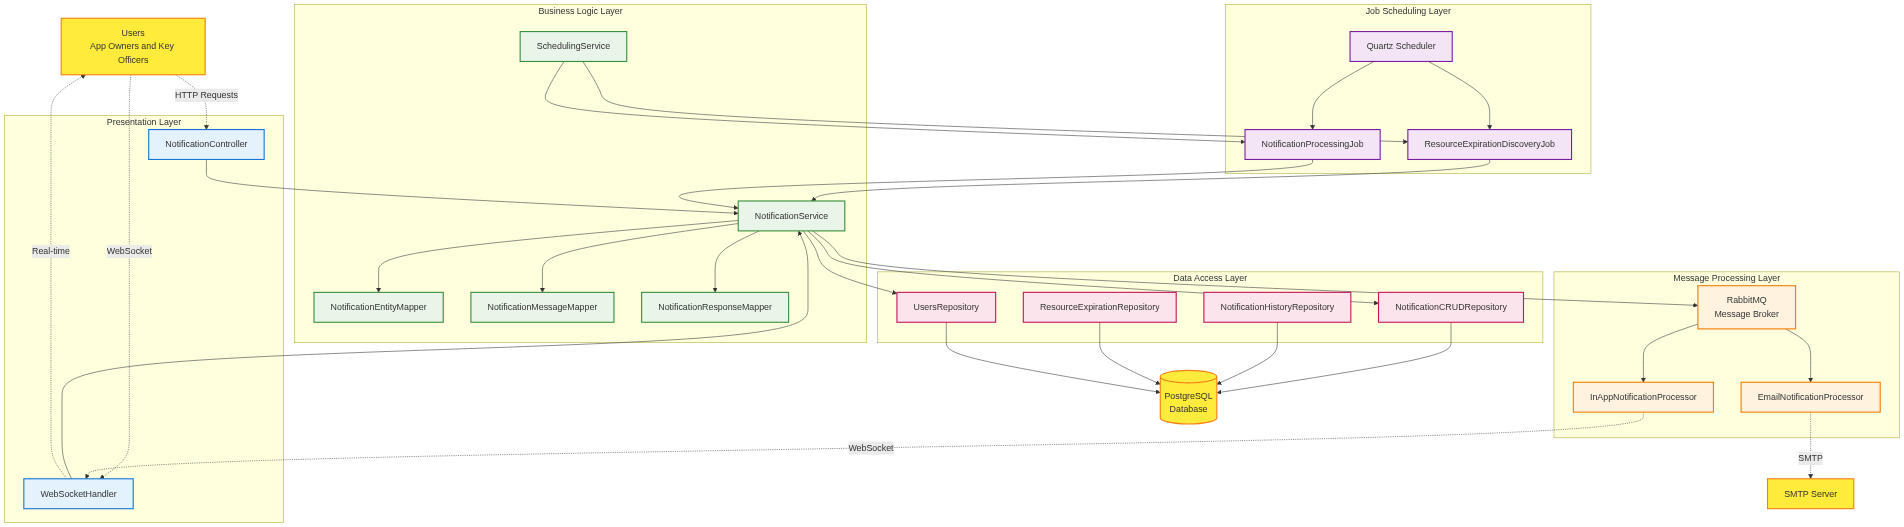
\includegraphics[width=1\textwidth]{images/system_architecture.png}
    \caption{System Architecture Overview}
    \label{fig:system_architecture}
\end{figure}

\textbf{Presentation Layer:}
\begin{itemize}
    \item \textbf{REST Controllers:} Handle HTTP requests and responses
        \begin{itemize}
            \item NotificationController: manages notification operations
            \item ManualSchedulingController: provides administrative functions
        \end{itemize}
    \item \textbf{WebSocket Handlers:} Manage real-time communication
        \begin{itemize}
            \item NotificationWebSocketHandler: handles in-app notifications
        \end{itemize}
\end{itemize}

\noindent
\textbf{Business Logic Layer:}
\begin{itemize}
    \item \textbf{Service Classes:} Implement core business logic
        \begin{itemize}
            \item NotificationService: manages notification lifecycle
            \item SchedulingService: handles manual job execution
        \end{itemize}
    \item \textbf{Mapper Classes:} Handle object transformations
\end{itemize}

\noindent
\textbf{Data Access Layer:}
\begin{itemize}
    \item \textbf{JPA Repositories:} Provide data persistence operations
        \begin{itemize}
            \item NotificationCRUDRepository: CRUD operations for notifications
            \item NotificationHistoryRepository: audit trail management
            \item ResourceExpirationRepository: resource discovery queries
        \end{itemize}
\end{itemize}

\noindent
\textbf{Message Processing Layer:}
\begin{itemize}
    \item \textbf{Message Processors:} Handle asynchronous notification delivery
        \begin{itemize}
            \item EmailNotificationProcessor: processes email notifications
            \item InAppNotificationProcessor: processes in-app notifications
        \end{itemize}
    \item \textbf{Message Queue:} RabbitMQ for reliable message delivery
\end{itemize}

\noindent
\textbf{Job Scheduling Layer:}
\begin{itemize}
    \item \textbf{Quartz Jobs:} Automated background processing
        \begin{itemize}
            \item ResourceExpirationDiscoveryJob: discovers expiring resources
            \item NotificationProcessingJob: processes scheduled notifications
        \end{itemize}
\end{itemize}

\subsection{Database Design}

\subsubsection{Database Schema}

The notification system extends the existing KMS database with two new entities designed to manage the complete lifecycle of expiration notifications.

\noindent
\textbf{Notification Entity:}
The primary entity that stores notification records with the following key attributes:

\noindent
\textbf{NotificationHistory Entity:}
An audit entity that preserves snapshots of notification state at the time of sending:

\noindent
These entities integrate seamlessly with existing KMS tables through foreign key relationships while maintaining data consistency and referential integrity.

\begin{figure}[H]
    \centering
    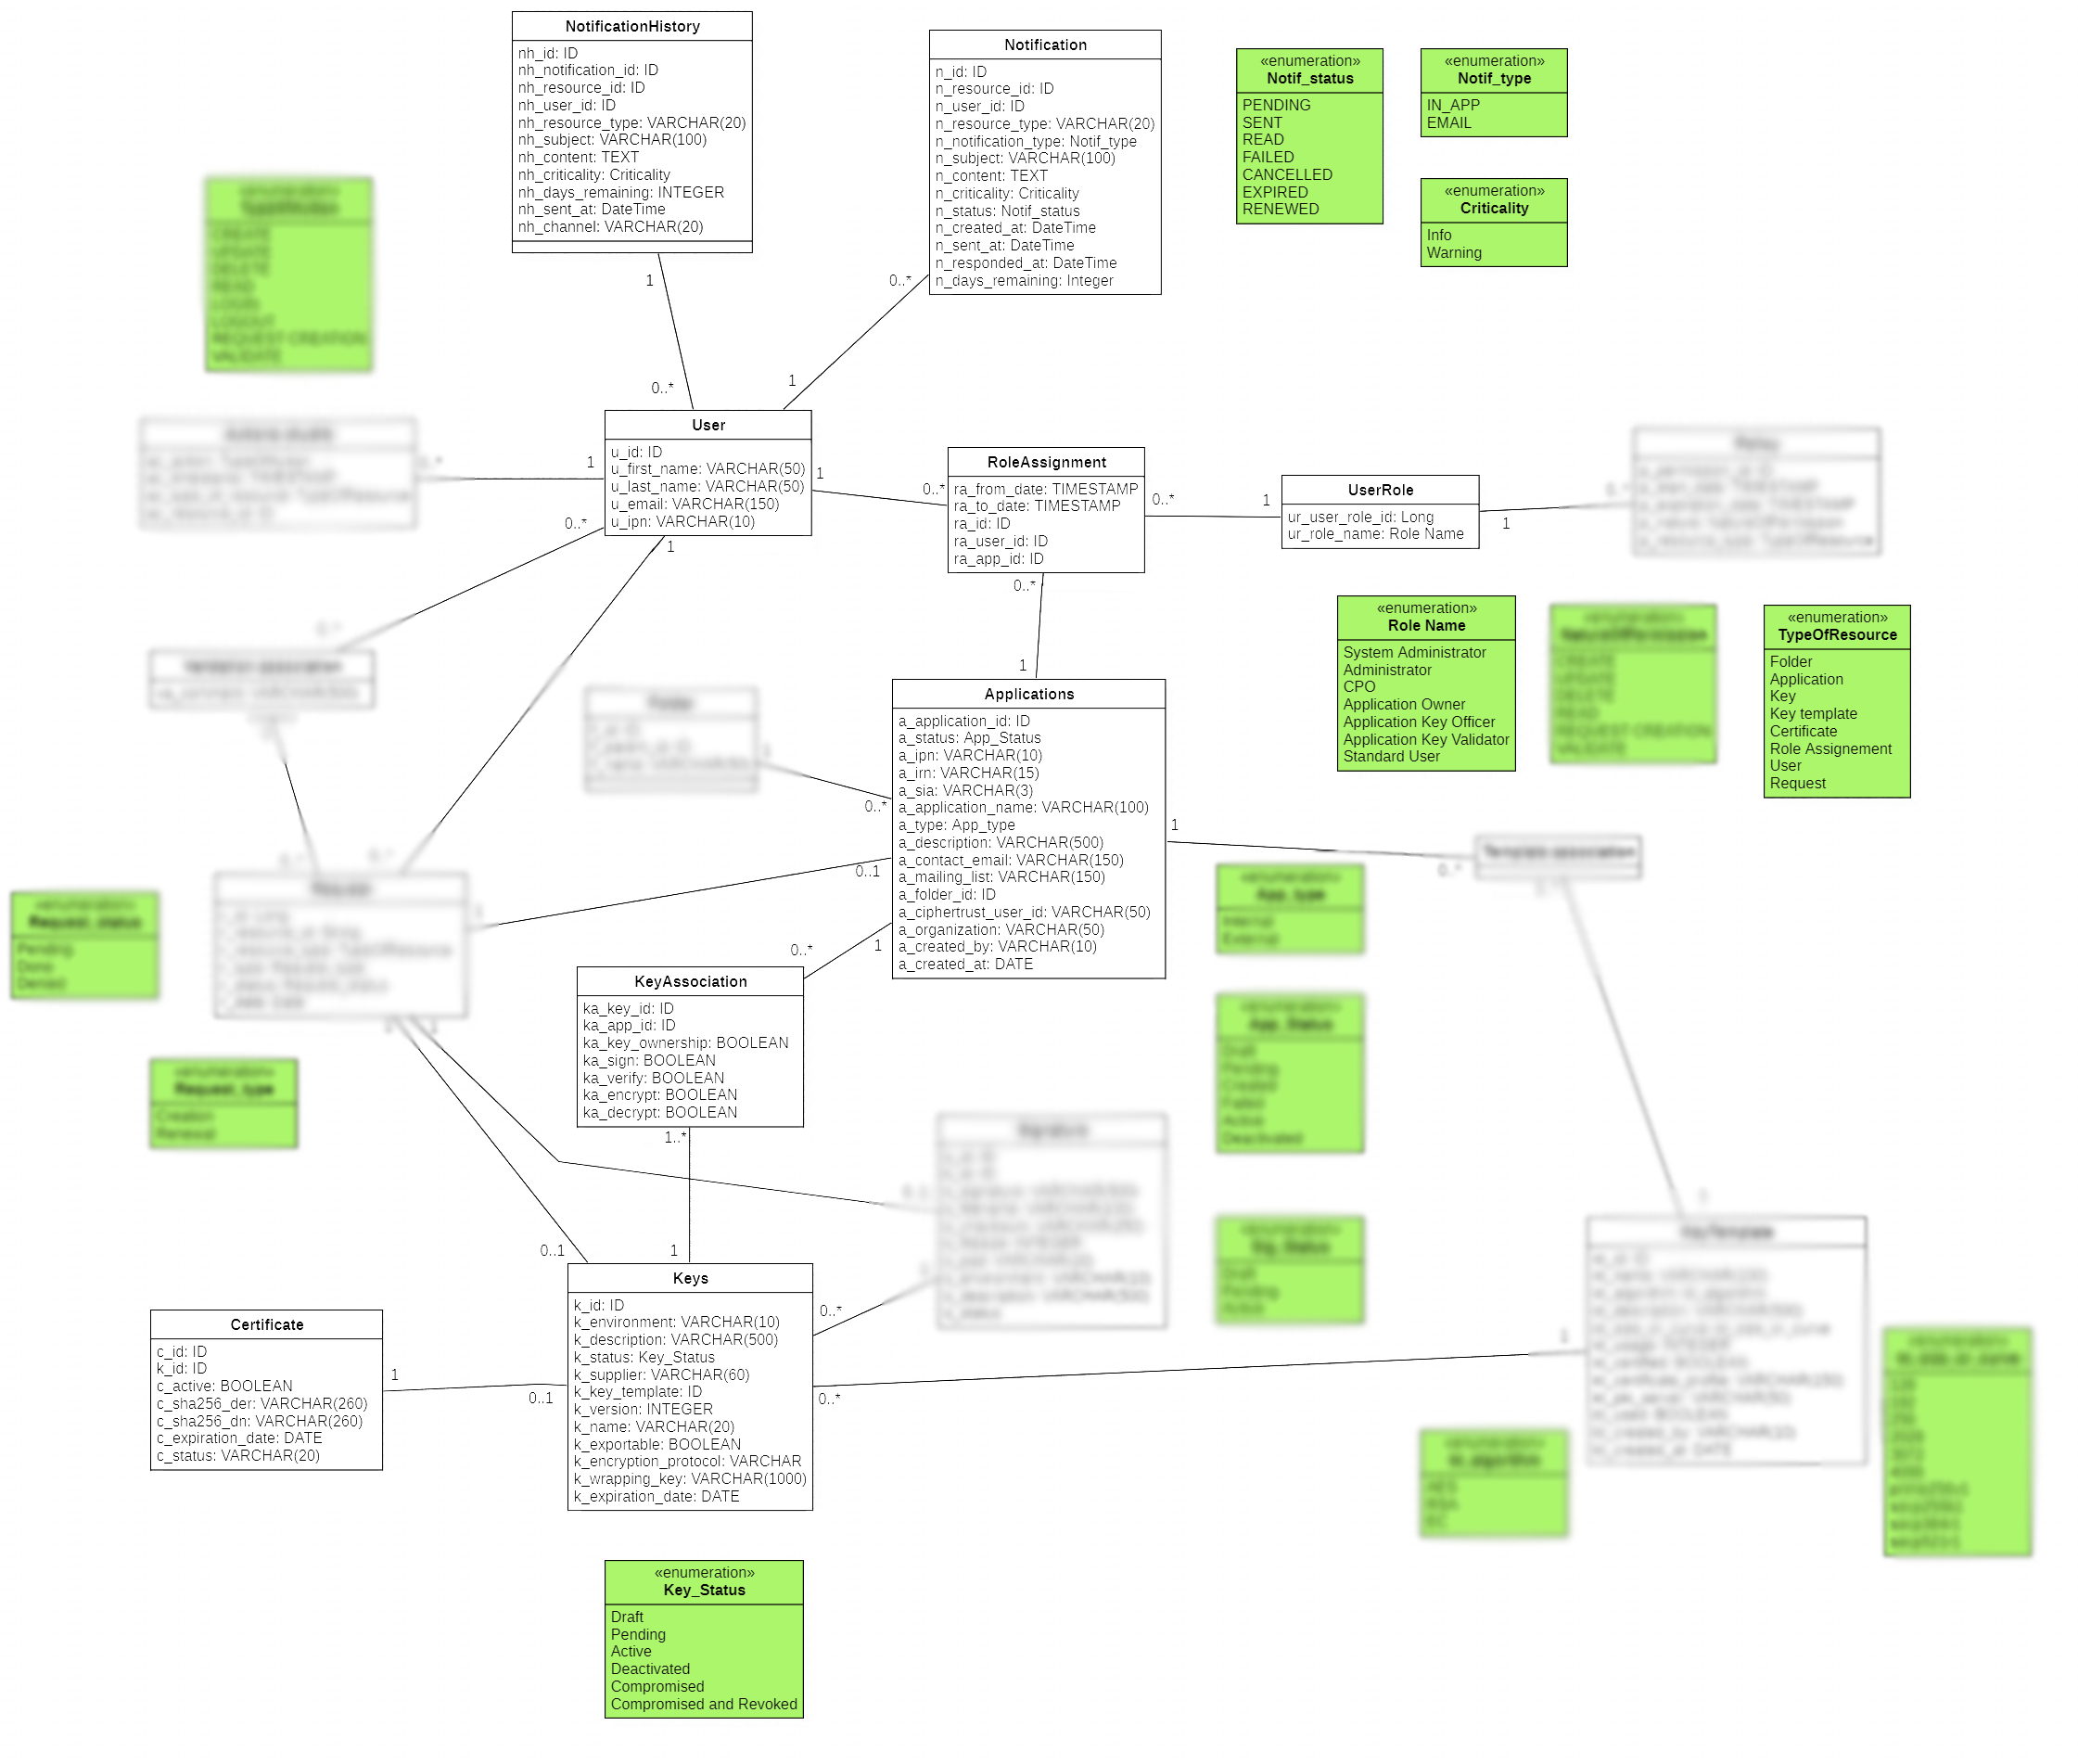
\includegraphics[width=1\textwidth]{images/database_schema.png}
    \caption{Database Schema}
    \label{fig:database_schema}
\end{figure}

\subsection{Component Design}

\subsubsection{Resource Discovery and Notification Processing}

The notification system operates through two distinct but interconnected processes: resource discovery and notification processing. These processes are implemented as separate Quartz jobs to ensure optimal performance and clear separation of concerns.

\newpage
\noindent
\textbf{Resource Discovery Process:}

% TODO: Insert Resource Discovery Diagram
\begin{figure}[H]
    \centering
    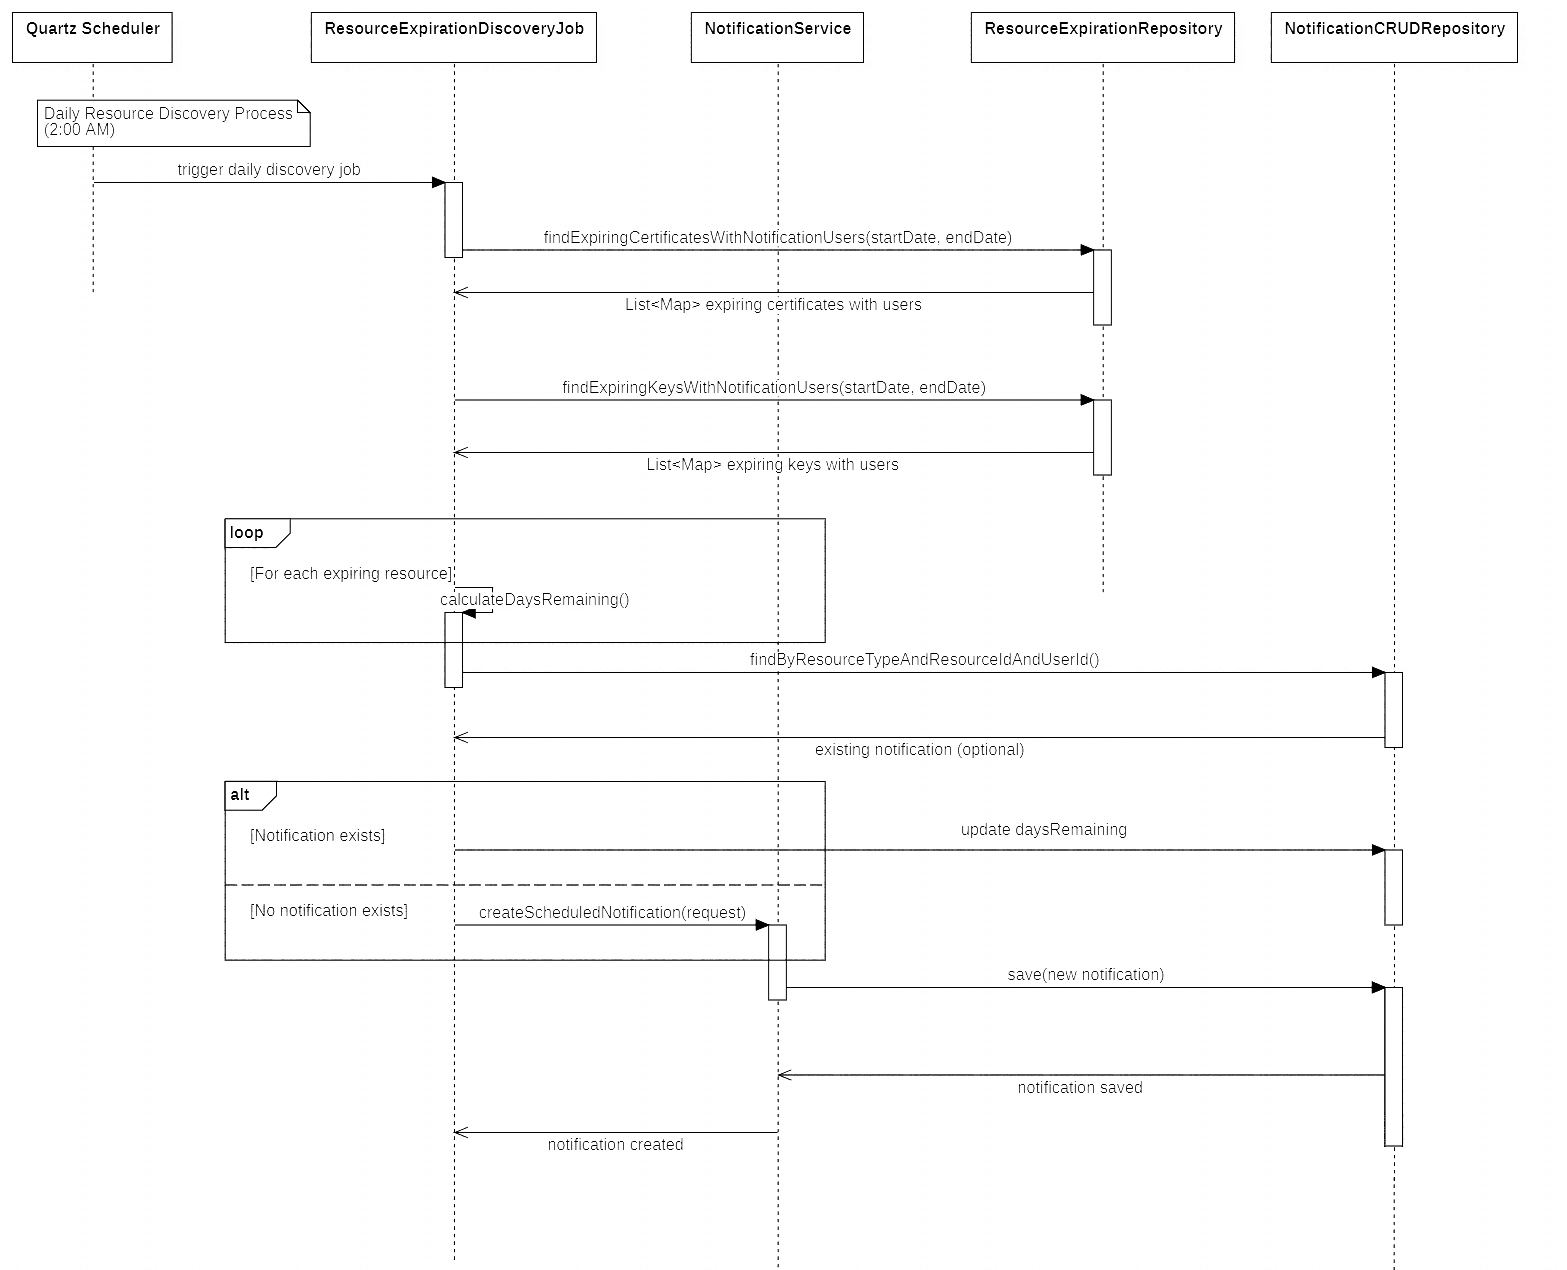
\includegraphics[width=1\textwidth]{images/resource_discovery_sequence.png}
    \caption{Resource Discovery Sequence Diagram}
    \label{fig:resource_discovery_sequence}
\end{figure}

\noindent
The ResourceExpirationDiscoveryJob executes daily at 2:00 AM to identify expiring cryptographic resources. The process queries both certificates and keys approaching expiration, identifies responsible users based on their role assignments, and creates or updates notification records. For existing notifications, the system updates the days remaining and resource status, while new expiring resources trigger the creation of scheduled notification records.

\newpage
\noindent
\textbf{Notification Processing and Delivery:}

% TODO: Insert Notification Processing Diagram
\begin{figure}[H]
    \centering
    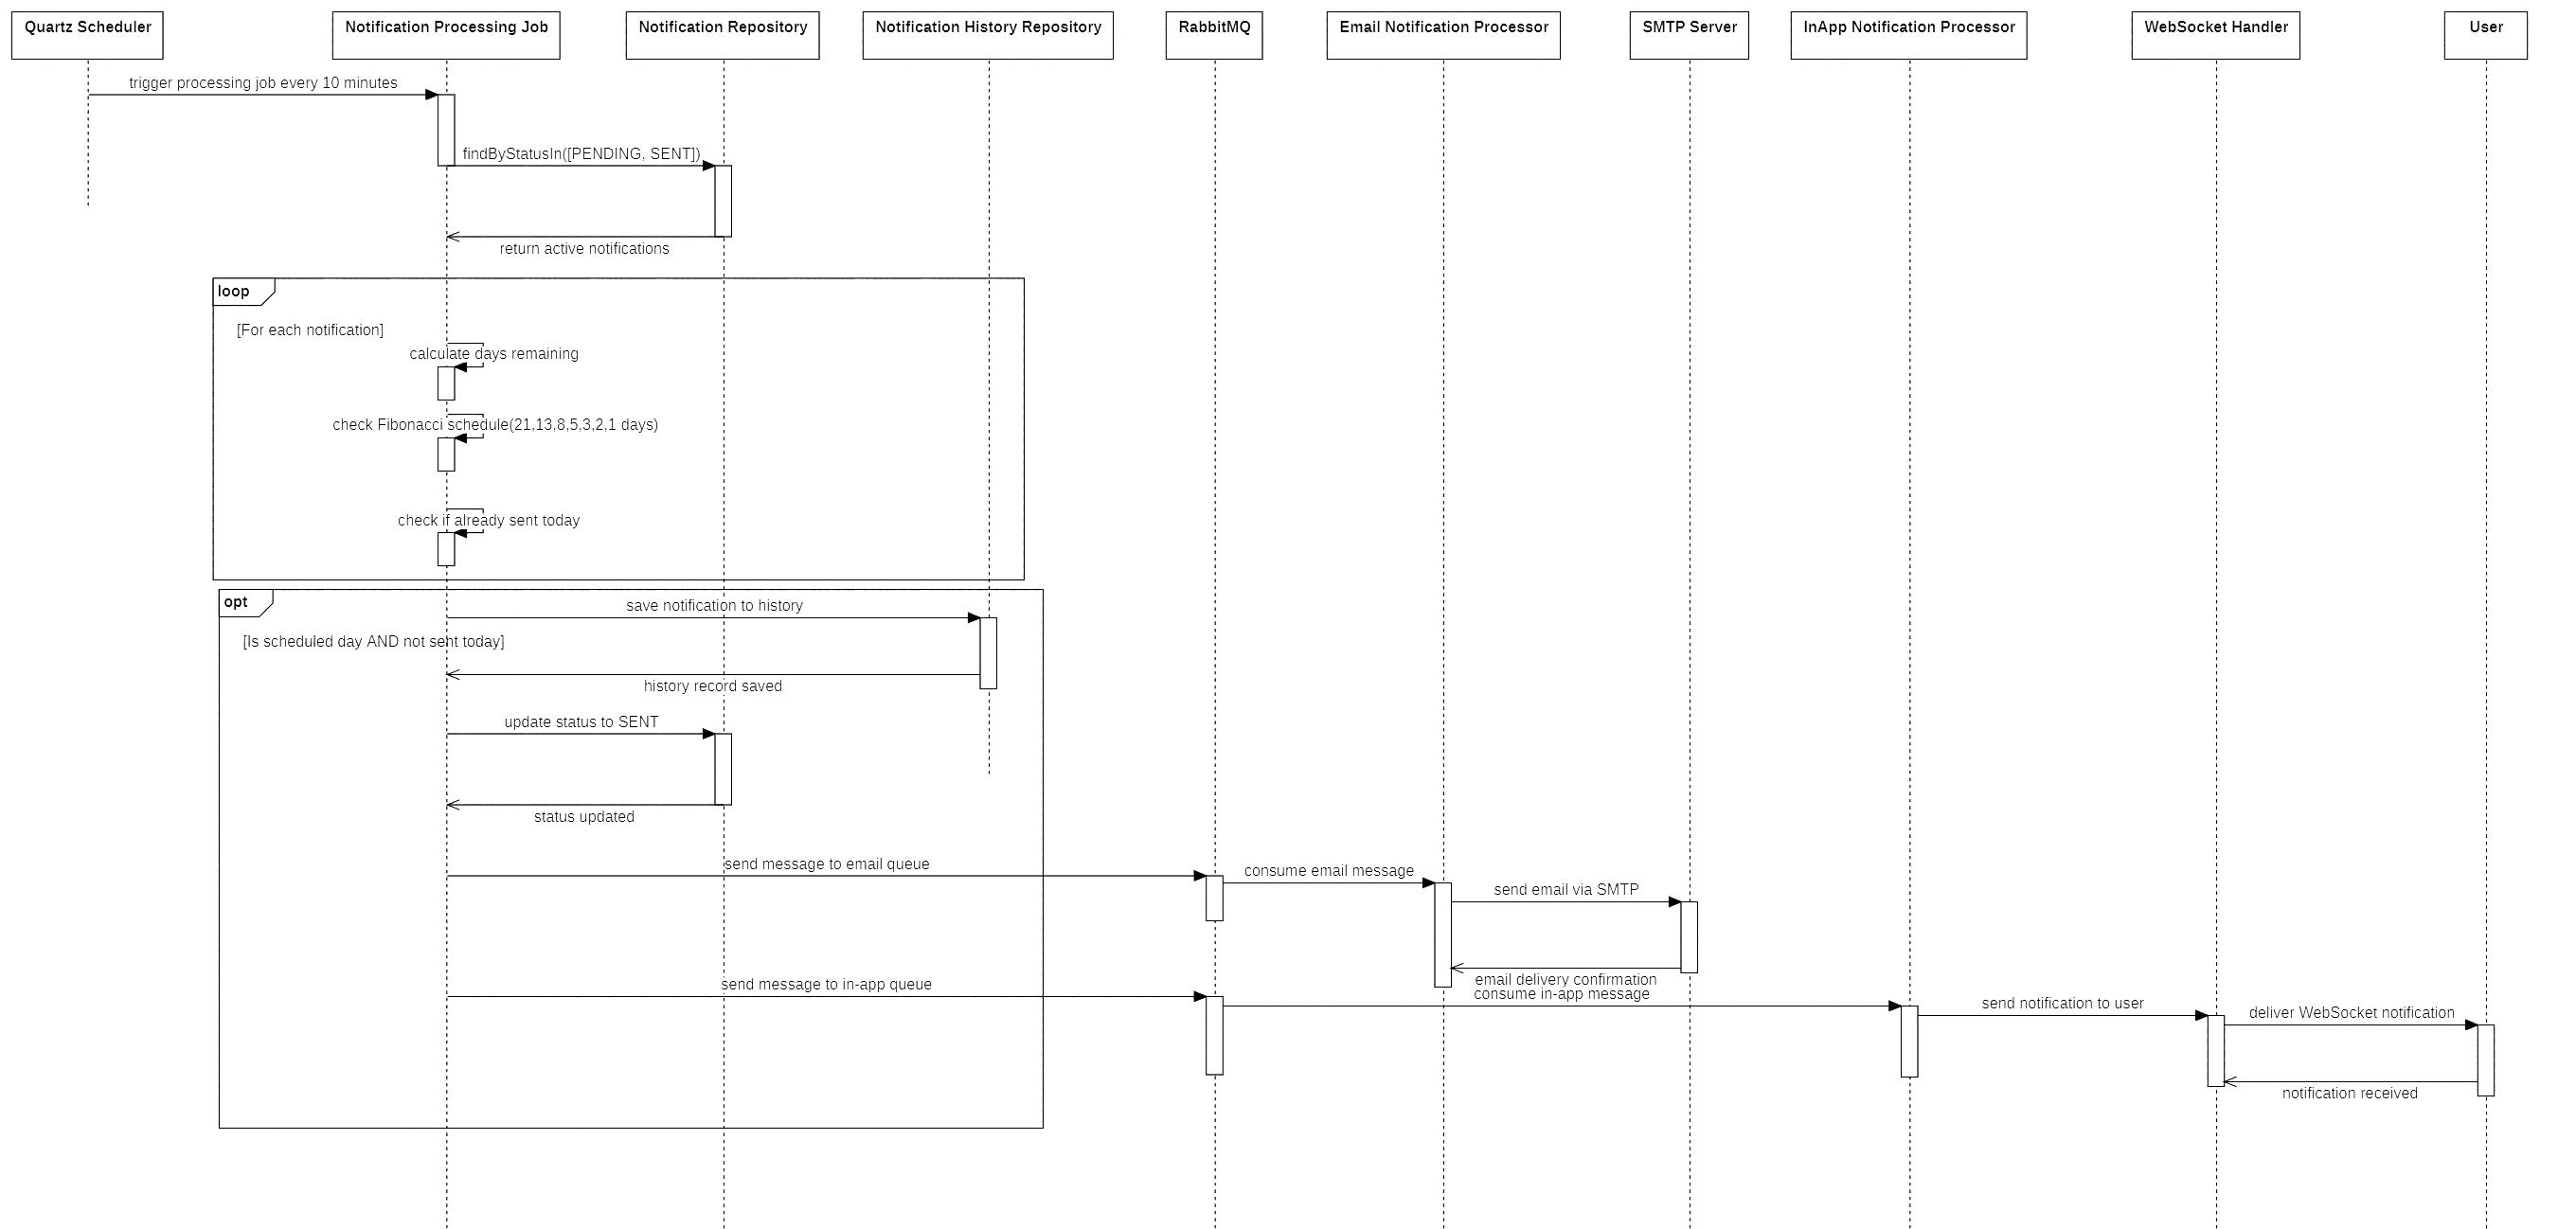
\includegraphics[width=1\textwidth]{images/notification_processing_sequence.png}
    \caption{Notification Processing and Delivery Sequence Diagram}
    \label{fig:notification_processing_sequence}
\end{figure}

\noindent
The NotificationProcessingJob executes every 10 minutes to process pending notifications using the Fibonacci scheduling algorithm (21, 13, 8, 5, 3, 2, 1 days before expiration). For notifications scheduled to be sent, the system saves a historical record, updates the notification status, and queues messages for both email and in-app delivery. The parallel processing architecture ensures that email notifications are sent via SMTP while in-app notifications are delivered through WebSocket connections, providing users with immediate awareness through multiple channels.\\

\noindent
\textbf{Scheduling Strategy:}

\noindent
The Fibonacci sequence provides an optimal balance between early warning and notification frequency. Users receive their first notification 21 days before expiration, with subsequent reminders following the mathematical sequence, creating increased urgency as the expiration date approaches while avoiding notification fatigue during the early warning period.

\newpage
\subsubsection{Message Queue Design}

% TODO: Insert RabbitMQ Architecture Diagram
\begin{figure}[H]
    \centering
    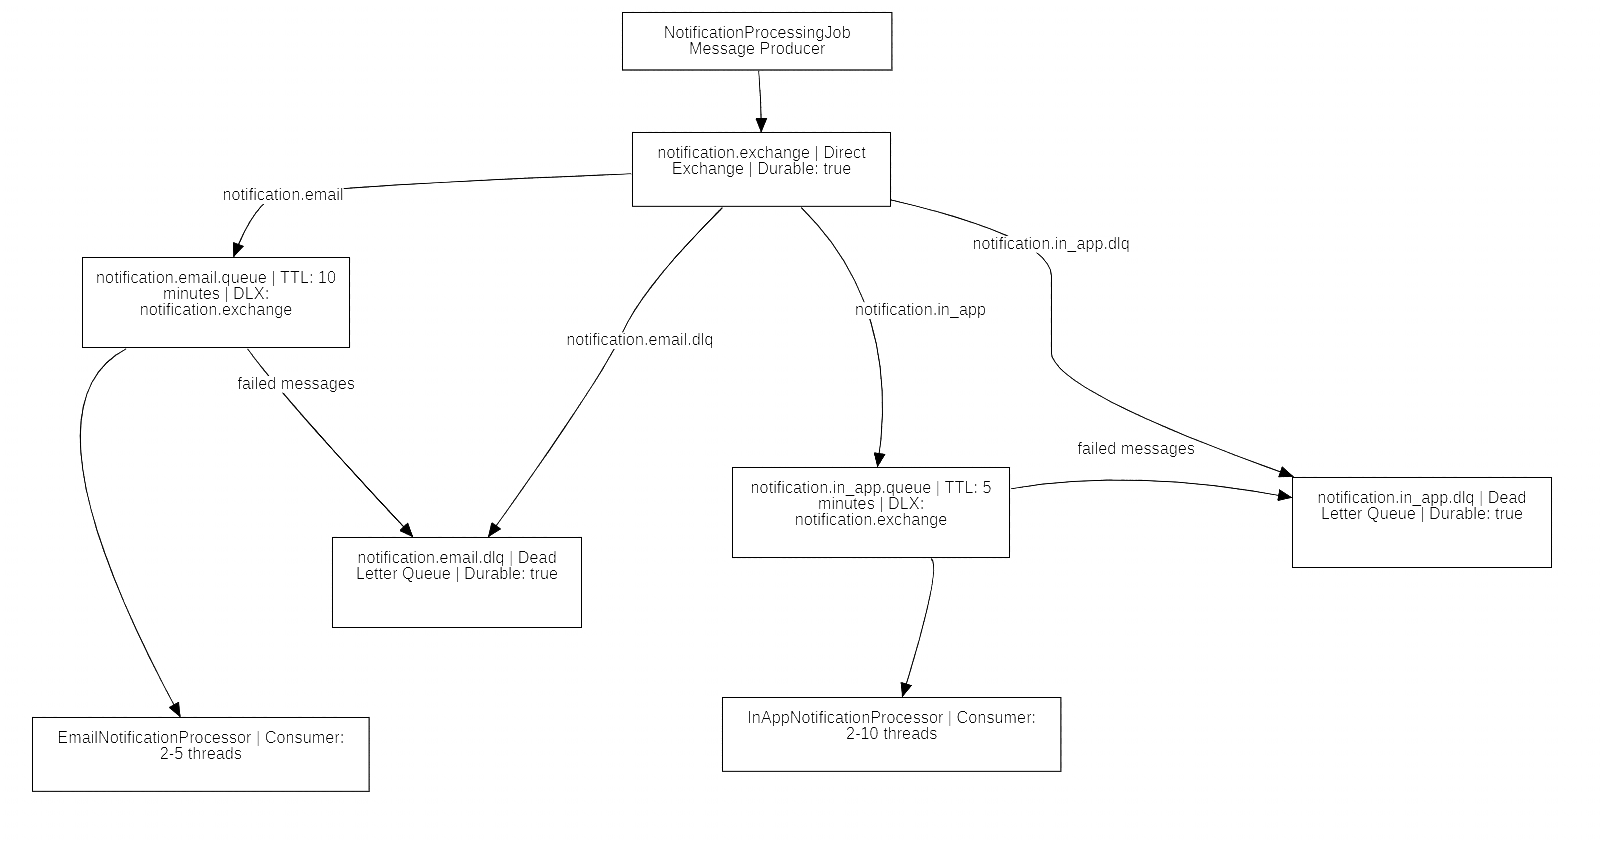
\includegraphics[width=1\textwidth]{images/rabbitmq_architecture.png}
    \caption{RabbitMQ Message Queue Architecture}
    \label{fig:rabbitmq_architecture}
\end{figure}

\textbf{Message Queue Architecture Design:}

\noindent
The notification system employs RabbitMQ as a message broker to ensure reliable and scalable message delivery through a carefully designed architecture. The system utilizes a \textbf{direct exchange} (notification.exchange), which routes messages to queues based on exact routing key matches, providing precise control over message distribution. When the NotificationProcessingJob publishes a message with routing key "notification.email", the direct exchange routes it exclusively to the email queue, while messages with "notification.in\_app" routing keys are directed to the in-app notification queue. This routing mechanism ensures clean separation between notification channels and prevents message misdelivery.

\noindent
To enhance system reliability, the architecture implements \textbf{dead letter queues} (DLQ) as a failure recovery mechanism. When messages in the primary queues exceed their time-to-live (TTL) limits or fail processing after maximum retry attempts, they are automatically redirected to their respective dead letter queues rather than being permanently lost. Email notifications have a 10-minute TTL to accommodate potential SMTP server delays, while in-app notifications use a shorter 5-minute TTL due to their real-time nature. The dead letter queues preserve failed messages for manual inspection and reprocessing, ensuring that critical expiration notifications are never permanently lost due to temporary system issues. This design provides both operational resilience and comprehensive audit capabilities, essential for maintaining the integrity of the cryptographic resource lifecycle management system.


\section*{Conclusion}

This chapter established the analytical foundation and design framework for the notification system within the KMS architecture. The requirements analysis identified the need for automated resource discovery, intelligent notification scheduling, and multi-channel communication to manage cryptographic resource lifecycles effectively.

\noindent
The system design presented a layered architecture promoting separation of concerns through distinct presentation, business logic, data access, message processing, and job scheduling layers. The database design integrates two new entities—Notification and NotificationHistory—with the existing KMS schema while enabling comprehensive audit capabilities. The component design detailed the workflow involving resource discovery jobs, Fibonacci-based scheduling algorithms, and parallel message processing through RabbitMQ infrastructure.

\noindent
This design foundation provides the blueprint for implementing an intelligent notification system that proactively manages cryptographic resource expirations, reducing operational risk and enhancing security compliance. The following chapter will detail the actual implementation of these design specifications.

\setcounter{chapter}{3}
\fancyhead[L]{Chapter III}
\fancyhead[R]{Implementation}

\vspace*{9cm}
\begin{doublespace}
    \centering
    \addcontentsline{toc}{chapter}{Chapter III: Implementation}
    \textbf{ \huge Chapter III \\ [1 cm] Implementation}
\end{doublespace} 

\newpage
\fancyhead[R]{\rightmark}

\setcounter{section}{0}
\section*{Introduction}

This chapter presents the practical implementation of the notification system within the KMS architecture. After establishing the requirements and design in the previous chapters, this phase focused on developing the actual REST API endpoints and WebSocket functionality that enable automated notification management for cryptographic resources. The implementation transforms the theoretical design into a working system, providing the necessary interfaces for users to interact with the notification system.

\section{Tools used}

\subsection{Software Resources:}

\vspace{0.5cm}

\noindent
\begin{minipage}{.7\textwidth}%
    \textbf{IntelliJ IDEA} is an integrated development environment (IDE) developed by JetBrains, mainly used for Java. It offers advanced features such as code auto-completion, project navigation, debugging, refactoring and integration with version control tools, which facilitates the development and maintenance of applications.
\end{minipage}%
\hfill
\begin{minipage}{.20\textwidth}%

\includegraphics[width=.8\textwidth]{images/intellij}
 \end{minipage} \\ \\ \\

\noindent% 
\begin{minipage}{.7\textwidth}%
    \textbf{Bruno} is an API testing and management tool, similar to Postman. It allows sending HTTP requests, analyzing responses and automating tests. Bruno is Git-friendly, and does not save data in the cloud, thus ensuring the confidentiality of information.
\end{minipage}%
\hfill
\begin{minipage}{.22\textwidth}%

\includegraphics[width=\textwidth]{images/bruno.png}
\end{minipage} \\ \\ \\

\noindent
\begin{minipage}{.7\textwidth}%
    \textbf{GitLab} is a web platform for managing Git repositories that allows code versioning, team collaboration and automation of development processes. It offers features such as issue tracking, continuous integration/continuous deployment (CI/CD) and branch management, thus facilitating the development, testing and deployment of software projects.
\end{minipage}%
\hfill
\begin{minipage}{.20\textwidth}%

\includegraphics[width=1\textwidth]{images/gitlab.png}
\end{minipage} \\ \\ \\ 

\noindent% 
\begin{minipage}{.7\textwidth}%
    \textbf{Git} is a version control system used to manage changes made to a computer project. It allows tracking changes, going back if necessary and collaborating effectively with other developers.
\end{minipage}%
\hfill
\begin{minipage}{.20\textwidth}%

\includegraphics[width=\textwidth]{images/git.png}
\end{minipage} \\ \\ \\

\noindent% 
\begin{minipage}{.7\textwidth}%
    \textbf{Rancher Desktop} is an application that allows easy management of container environments on a development workstation. It integrates Kubernetes and containerization tools like containerd or Docker, allowing to create, test and deploy containerized applications locally before sending them to production. Rancher Desktop thus facilitates learning and experimentation with cloud and microservices technologies.
\end{minipage}%
\hfill
\begin{minipage}{.18\textwidth}%

\includegraphics[width=\textwidth]{images/rancher.png}
\end{minipage} \\ \\ \\

\noindent% 
\begin{minipage}{.7\textwidth}%
    \textbf{PostgreSQL} is a powerful and reliable open-source relational database management system. It supports standard SQL and offers advanced features such as transactions, views, stored procedures and extension via custom data types. PostgreSQL is particularly appreciated for its robustness, standards compliance and ability to efficiently handle large amounts of data.
\end{minipage}%
\hfill
\begin{minipage}{.18\textwidth}%

\includegraphics[width=\textwidth]{images/postgresql.png}
\end{minipage} \\ \\ \\

\subsection{Programming languages:}

\vspace{0.5cm}

\noindent% 
\begin{minipage}{.7\textwidth}%
    \textbf{Java} is an object-oriented, versatile and widely used programming language, developed by Sun Microsystems in 1995 (now owned by Oracle). It is designed to be portable, secure and robust, making it a popular choice for developing a variety of applications, from desktop applications to embedded systems through web and mobile applications.
\end{minipage}%
\hfill
\begin{minipage}{.20\textwidth}%

\includegraphics[width=\textwidth]{images/java.png}
\end{minipage} \\ \\ \\ 

\subsection{Frameworks and libraries:}

\vspace{0.5cm}

\noindent% 
\begin{minipage}{.7\textwidth}%
    \textbf{Spring Boot} is a Java framework that simplifies the development of standalone and production-ready applications. It provides automatic configuration, integrated dependencies and tools to quickly create web services, REST APIs and microservices applications, while reducing boilerplate code and facilitating deployment.
\end{minipage}%
\hfill
\begin{minipage}{.20\textwidth}%

\includegraphics[width=\textwidth]{images/spring_boot.png}
\end{minipage} \\ \\ \\

\section{REST API Implementation}

The notification system exposes a comprehensive REST API that enables immediate notification sending, scheduled notification management, and resource status updates. The API follows RESTful principles and integrates seamlessly with the existing KMS architecture.

\subsection{Immediate Notification Endpoint}

The immediate notification endpoint provides the capability to send notifications instantly to users through both email and in-app channels. This endpoint serves as a critical safety mechanism that bypasses the automated Fibonacci scheduling system for emergency situations.

\subsubsection{Purpose and Use Cases}

The immediate notification functionality addresses several critical scenarios that require instant user alerting:

\noindent
\textbf{Emergency Situations:} When cryptographic resources expire unexpectedly soon due to configuration errors or system issues, waiting for the next scheduled processing cycle (every 10 minutes) may be too late. The immediate endpoint ensures that critical alerts reach responsible users within seconds.

\noindent
\textbf{Administrative Interventions:} System administrators can manually trigger notifications for specific resources that may not have been captured by the automated discovery process, or when manual oversight identifies critical situations requiring immediate attention.

\noindent
\textbf{Testing and Validation:} The endpoint serves as a testing mechanism to verify that notification channels are functioning correctly and that users can receive real-time alerts through both email and WebSocket connections.

\subsubsection{Immediate vs Scheduled Notification Flow}

The notification system implements two distinct processing flows:

\noindent
\textbf{Scheduled Flow (Normal Operations):}
Discovery Job → Creates notification records → Processing Job (Fibonacci schedule) → Sends notifications

\noindent
\textbf{Immediate Flow (Emergency/Manual Operations):}
API Call → Instant notification delivery to EMAIL + IN\_APP channels

This dual approach ensures that while the system operates efficiently through automated scheduling for regular expiration management, it maintains the flexibility to handle urgent situations that require immediate user notification.

\subsubsection{Endpoint Specification}

\textbf{POST /v1/notifications/immediate}

This endpoint accepts an immediate notification request and triggers instant delivery through available notification channels. The request requires resource identification, user targeting, and notification content.

\noindent
\textbf{Request Body Structure:}
\begin{itemize}
    \item \textbf{resourceId}: Unique identifier of the cryptographic resource
    \item \textbf{userId}: Target user identifier
    \item \textbf{resourceType}: Type of resource (Certificate or Key)
    \item \textbf{subject}: Notification subject line
    \item \textbf{message}: Detailed notification content
\end{itemize}

\noindent
\textbf{Response:} Returns a list of notification response objects containing the created notification details and delivery status for each enabled channel.

\subsubsection{API Testing with Bruno}

The immediate notification endpoint was thoroughly tested using Bruno to validate request processing and response handling.

\begin{figure}[H]
    \centering
    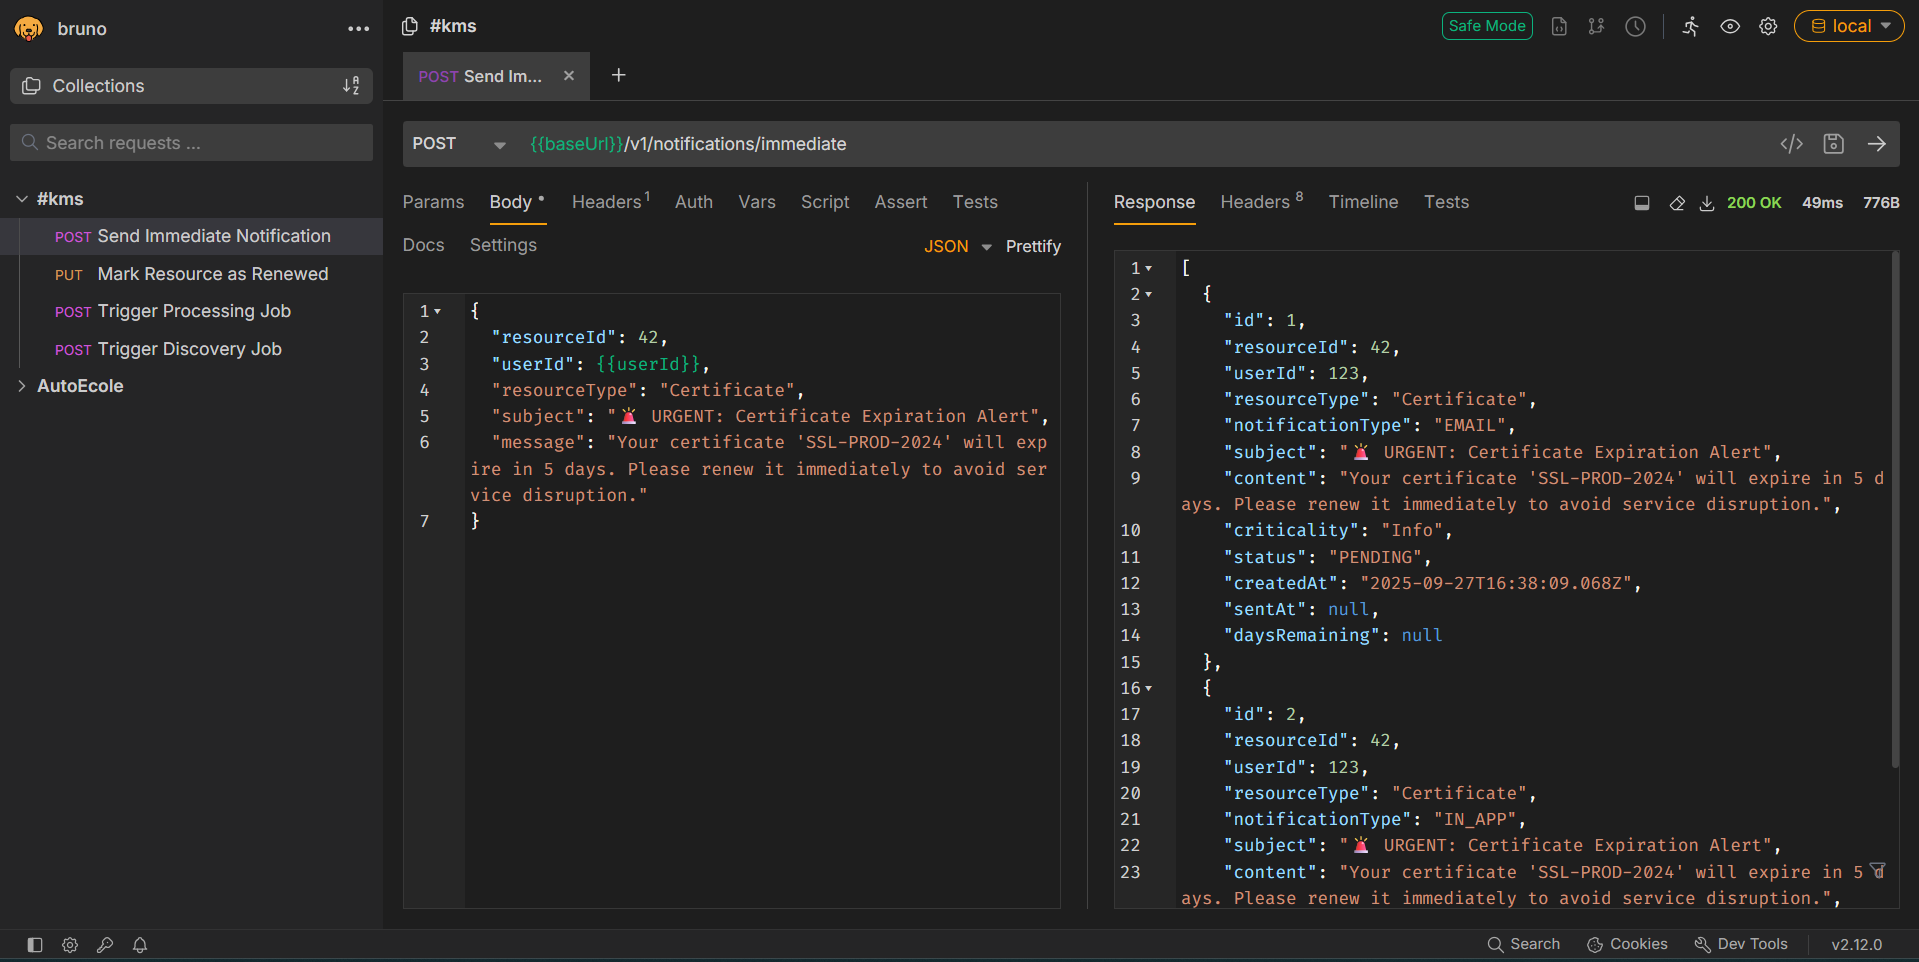
\includegraphics[width=1\textwidth]{images/bruno_immediate_notification.png}
    \caption{Bruno Testing - Immediate Notification Request and Response}
    \label{fig:bruno_immediate}
\end{figure}

The test demonstrates successful processing of an immediate notification request. The response confirms that notifications were created for both email and in-app channels, with unique notification IDs assigned to each channel. The status "PENDING" indicates that the notifications have been queued for processing.

\subsection{Resource Response Endpoint}

This endpoint allows users to mark cryptographic resources as renewed or responded to, which automatically cancels future notifications for those resources.

\subsubsection{Endpoint Specification}

\textbf{PUT /v1/notifications/resource/\{resourceId\}/\{resourceType\}/responded}

This endpoint updates the status of all active notifications for a specific resource, marking them as cancelled when a user indicates they have taken action on the expiring resource.

\noindent
\textbf{Path Parameters:}
\begin{itemize}
    \item \textbf{resourceId}: Unique identifier of the resource
    \item \textbf{resourceType}: Type of the resource (Certificate or Key)
\end{itemize}

\noindent
\textbf{Response:} Returns a confirmation message indicating successful status update.

\subsubsection{Testing Resource Response}

\begin{figure}[H]
    \centering
    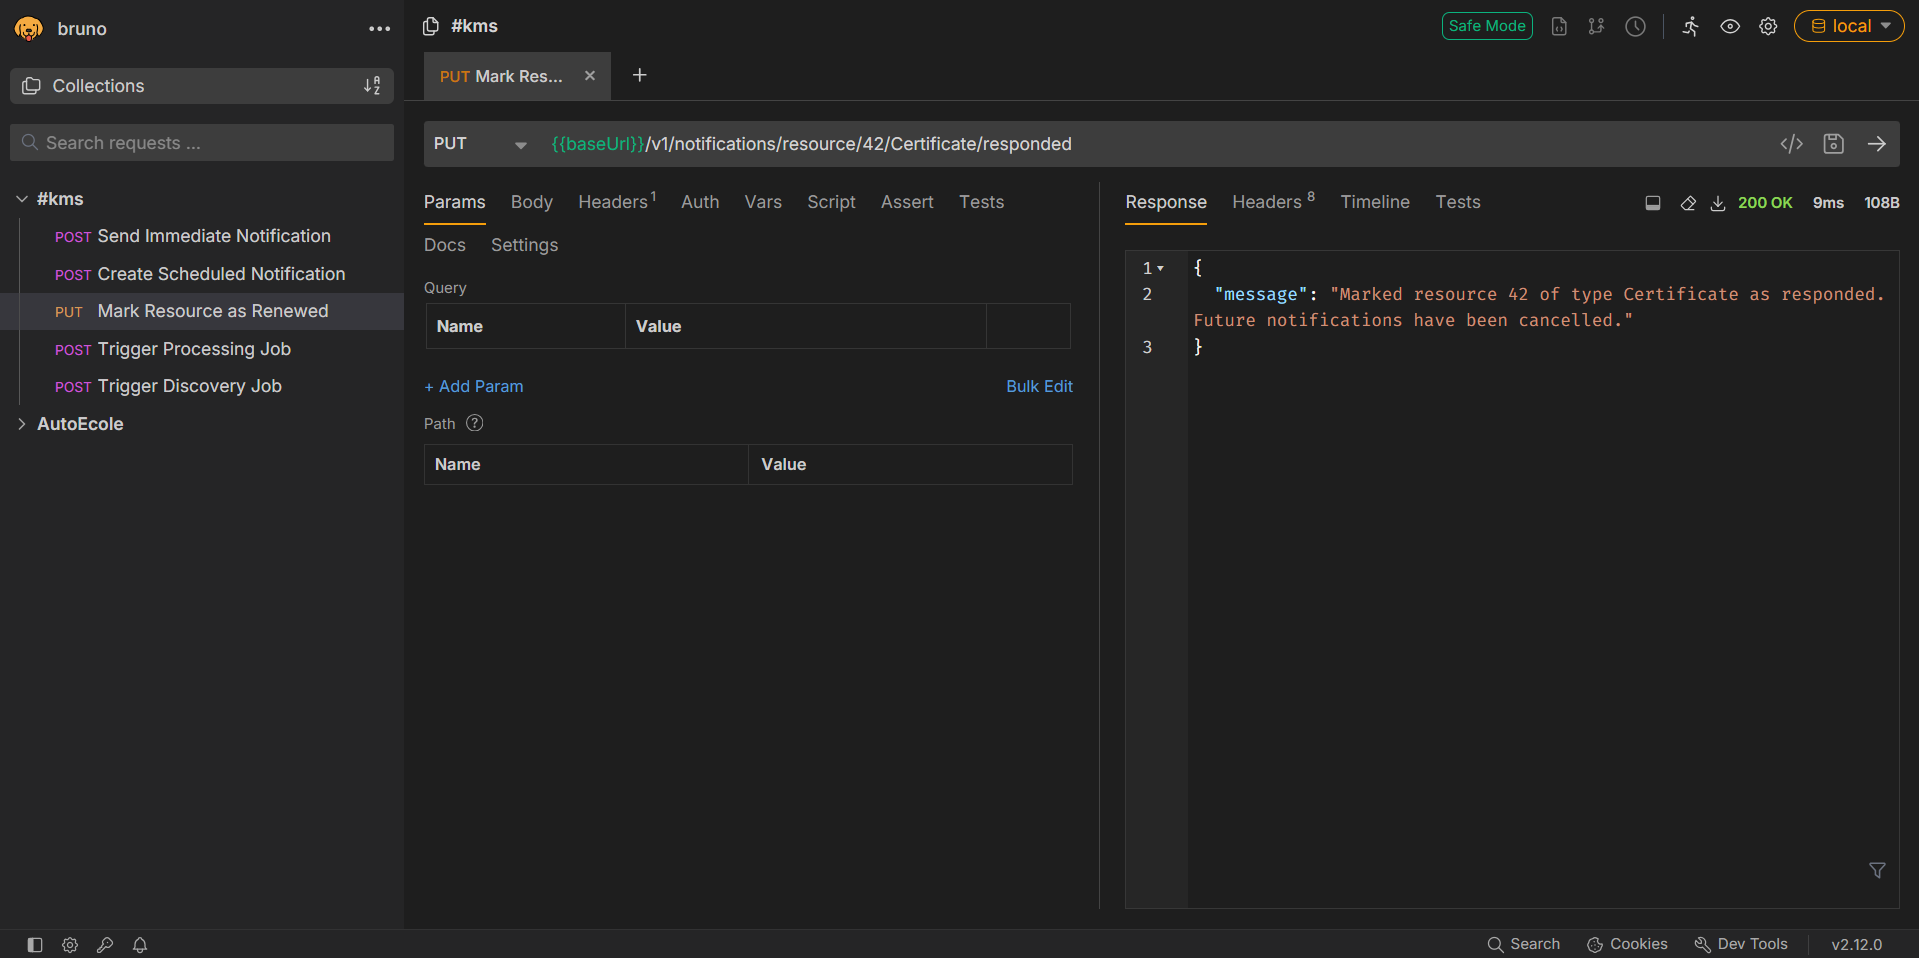
\includegraphics[width=1\textwidth]{images/bruno_resource_response.png}
    \caption{Bruno Testing - Mark Resource as Renewed}
    \label{fig:bruno_resource_response}
\end{figure}

The test confirms that the endpoint successfully processes resource response requests, updating notification statuses and preventing unnecessary future notifications.

\section{WebSocket Implementation}

The WebSocket implementation enables real-time delivery of in-app notifications, providing users with immediate awareness of expiring cryptographic resources.

\subsection{WebSocket Connection Setup}

The WebSocket endpoint is configured to accept connections with user identification, enabling targeted message delivery to specific users.

\subsubsection{Connection Endpoint}

\textbf{WebSocket URL: ws://localhost:8080/ws/notifications?userId=\{userId\}}

The connection requires a userId parameter to identify the target user for notification delivery. Upon successful connection, the system maintains the session and can deliver real-time notifications to the connected user.

\subsection{WebSocket Testing}

Real-time notification delivery was validated using a custom HTML test page that demonstrates WebSocket connectivity and message reception.

\subsubsection{Connection Establishment}

\begin{figure}[H]
    \centering
    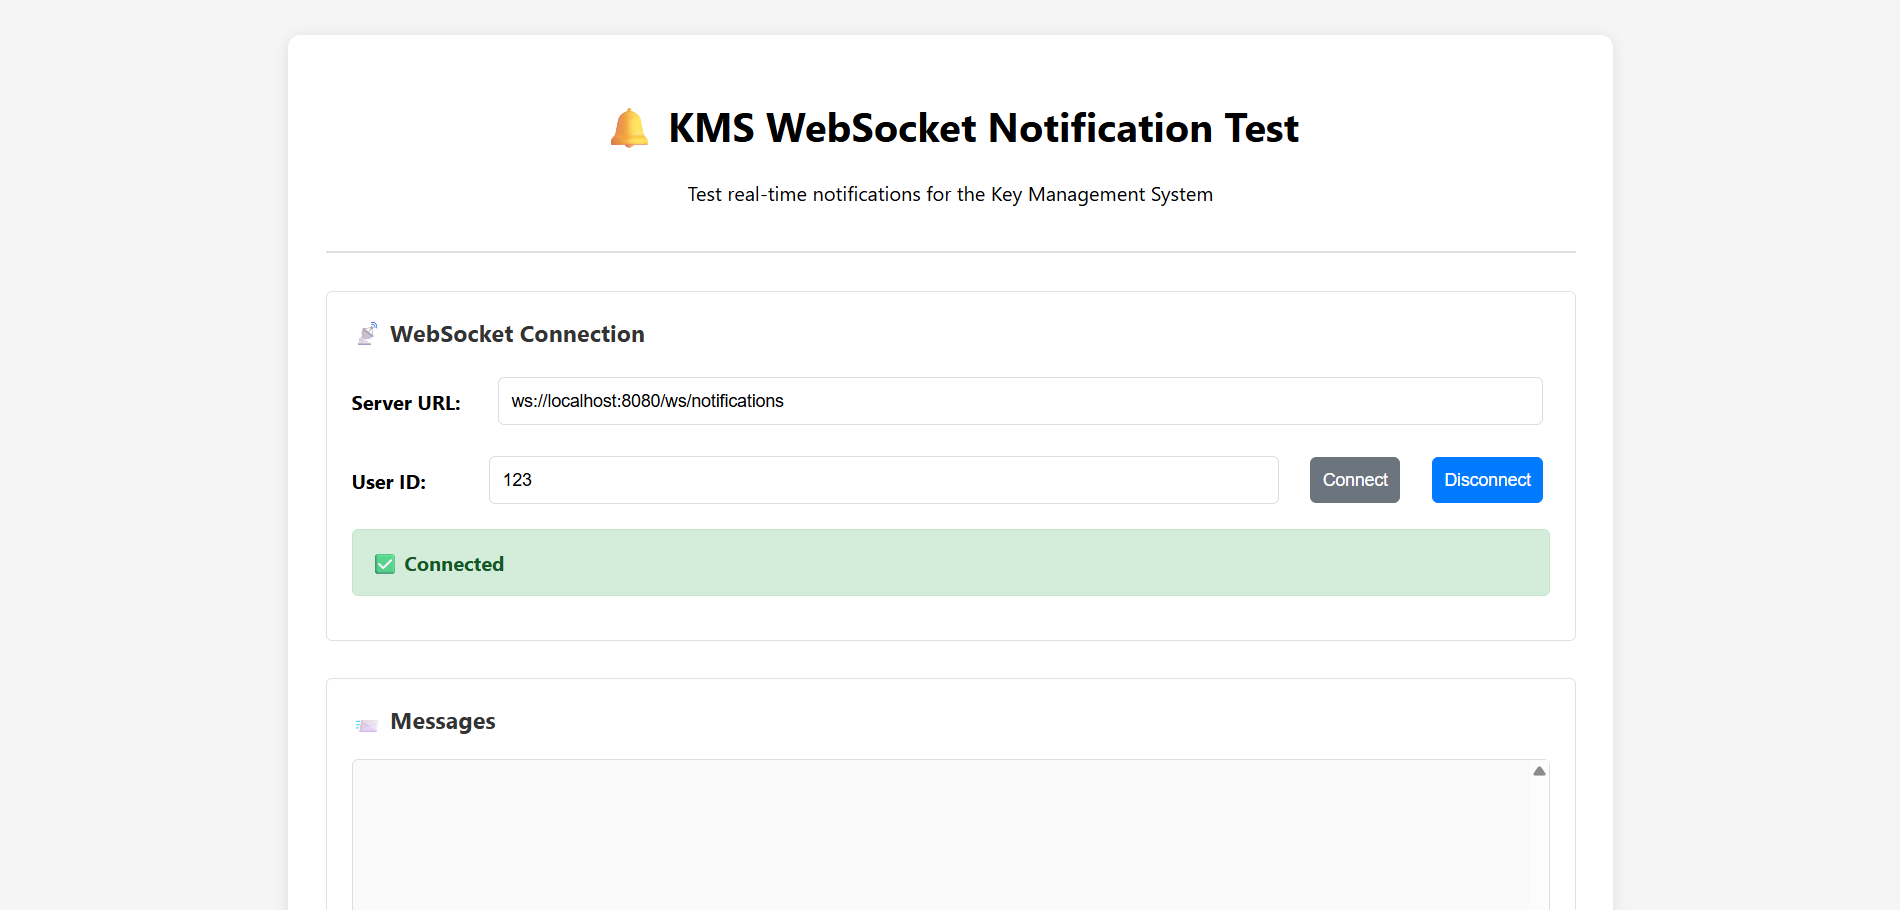
\includegraphics[width=1\textwidth]{images/websocket_connection.png}
    \caption{WebSocket Connection Test Interface}
    \label{fig:websocket_connection}
\end{figure}

The test interface shows successful WebSocket connection establishment with proper user identification. The connection status indicates active communication channel for real-time notification delivery.

\subsubsection{Real-time Message Delivery}

\begin{figure}[H]
    \centering
    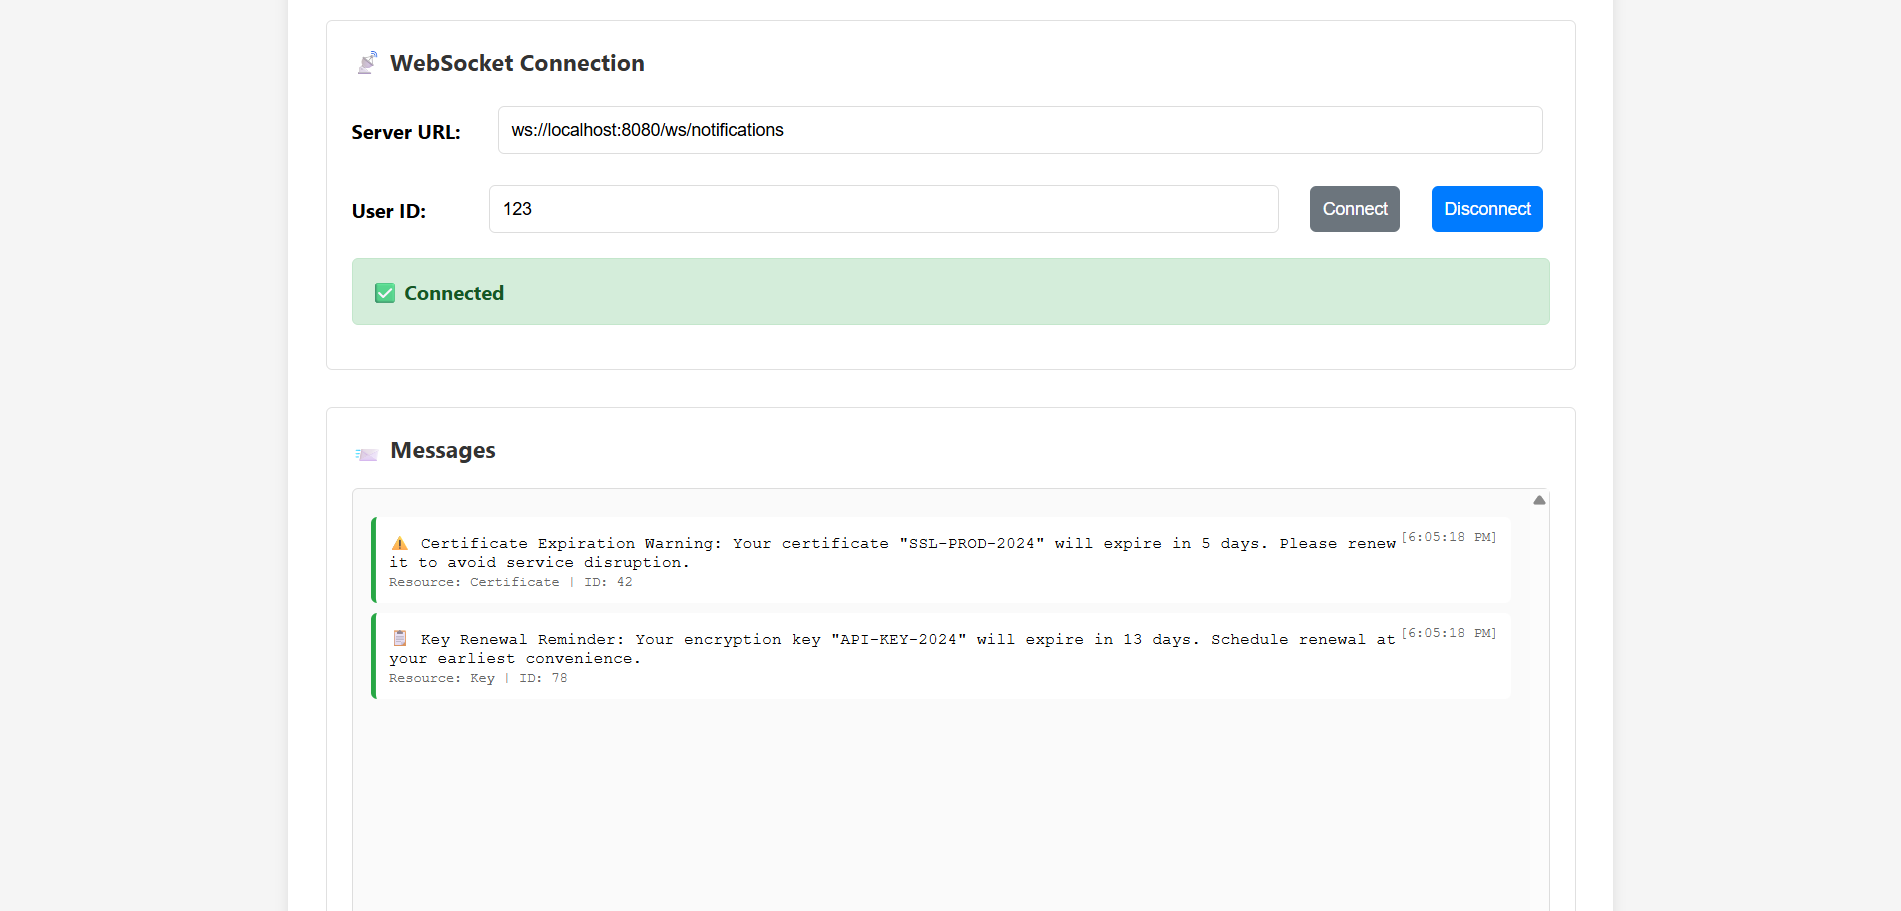
\includegraphics[width=1\textwidth]{images/websocket_message.png}
    \caption{WebSocket Real-time Notification Delivery}
    \label{fig:websocket_message}
\end{figure}

The message delivery test demonstrates successful real-time notification transmission through the WebSocket connection. The structured message format includes notification details, resource information, and timing data, providing users with comprehensive information about expiring cryptographic resources.

\section{Manual Job Execution Endpoints}

For testing and administrative purposes, the system provides endpoints to manually trigger the background jobs that normally run on scheduled intervals.

\subsection{Process Notifications Endpoint}

\textbf{POST /v1/notifications/jobs/process-notifications}

This endpoint manually triggers the notification processing job, which evaluates pending notifications and sends those matching the current day in the Fibonacci sequence.

\subsection{Resource Discovery Endpoint}

\textbf{POST /v1/notifications/jobs/discover-all-resources}

This endpoint manually triggers the resource discovery job, which scans the database for expiring certificates and keys and creates appropriate notification records.

These administrative endpoints proved essential during development and testing phases, allowing for controlled execution of the automated processes.

\section*{Conclusion}

This chapter presented the practical implementation of the notification system, focusing on the development of REST API endpoints and WebSocket functionality. The implementation successfully provides the necessary interfaces for immediate and scheduled notification management, resource status updates, and real-time communication.

The use of modern development tools and frameworks facilitated efficient implementation while maintaining code quality and system reliability. The comprehensive API testing with Bruno validated endpoint functionality and request/response handling, ensuring that the system meets the specified requirements.

The WebSocket implementation adds real-time capability to the notification system, enhancing user experience by providing immediate awareness of critical resource expirations. The combination of REST APIs and WebSocket communication creates a comprehensive notification platform that addresses both immediate and long-term cryptographic resource management needs.

The implemented endpoints integrate seamlessly with the existing KMS architecture while providing the foundation for automated notification processes described in the previous chapters. This implementation represents a significant step toward proactive cryptographic resource lifecycle management within the Renault Group's security infrastructure.
 
\addcontentsline{toc}{chapter}{General conclusion}
\fancyhead{}

\vspace*{1cm}
\begin{center}
    \textbf{\huge{General Conclusion}}
\end{center}
\vspace{1cm}

\begin{doublespace}
This internship at Renault Digital Morocco provided valuable hands-on experience in enterprise software development within the cybersecurity domain. Working on the Key Management System allowed for practical application of modern Java technologies and agile development methodologies in a real-world industrial context.

The project highlighted the importance of understanding business requirements beyond technical specifications. Developing a notification system required careful consideration of user workflows, organizational roles, and operational constraints—demonstrating that effective software solutions must balance technical capabilities with human factors.

From a technical perspective, the integration of multiple technologies—Spring Boot, message queuing, WebSocket communication, and database design—reinforced the complexity of enterprise application development. The experience emphasized the value of modular architecture and the challenges of maintaining system reliability in production environments.

This internship strengthened both technical skills and professional competencies, particularly in requirements analysis, system design, and collaborative development. The exposure to Renault's engineering practices and quality standards provides a solid foundation for future career development in enterprise software engineering.

The project serves as a practical example of how targeted automation can address specific operational needs while contributing to broader organizational objectives in security and compliance.
\end{doublespace}

\vspace*{1cm}
\begin{center}
    \textbf{\huge{Bibliography}}
\end{center}

\vspace*{0.5cm}

\begin{itemize}
    \item \url{https://spring.io/projects/spring-boot} (accessed August 15, 2025)
    
    \item \url{https://www.rabbitmq.com/tutorials} (accessed August 18, 2025)

    \item \url{https://docs.spring.io/spring-framework/docs/current/reference/html/web.html#websocket} (accessed August 20, 2025)

    \item \url{https://docs.spring.io/spring-data/jpa/docs/current/reference/html/} (accessed August 25, 2025)

    \item \url{https://www.quartz-scheduler.org/documentation/} (accessed August 28, 2025)

    \item \url{https://www.atlassian.com/agile/scrum} (accessed August 5, 2025)

    \item \url{https://spring.io/guides/gs/messaging-rabbitmq/} (accessed August 19, 2025)

\end{itemize}

\end{document}